%%%%%%%%%%%%%%%%%%%%%%%%%%%%%
%ES100 Latex Template
%Sam Meijer '19
%Hopefully this template will serve you well.
%It is built off many other packages and templates, but I have added my own style here and there, as you should too!
%I will endeavour to explain some of the intricacies of LaTex as well as how to lay out an overall project.
%Hopefully no knowledge of LaTex is required to understand this document.
%I would highly recommend https://www.overleaf.com/learn/latex/Main_Page for further information.
%For errata, please contact smeijer11@gmail.com.
%%%%%%%%%%%%%%%%%%%%%%%%%%%%%

%Packages are included below, these are akin to libraries in other programming languages. As far as I can tell, there is no reason to reduce the number of packages included in a document. It might compile faster, but overleaf compiles fast so this should not be an issue.
\documentclass[12pt,twoside, notitlepage]{article}%tells the compiler that this is a 'report' style document, and the main font size.
\IEEEoverridecommandlockouts
\usepackage{setspace} %allows the use of '\doublespace' to set line spacing
\usepackage[utf8]{inputenc} %inclusion of this is optional, overleaf includes it in its compiler so it is not necessary, it may be necessary for other compilers.
\usepackage[english]{babel} %this does a few things eg allowing dates to be made by the compiler. probably best not to get rid of it
\usepackage{wrapfig} %if it is desirable to wrap text (see https://www.overleaf.com/learn/latex/Wrapping_text_around_figures).
\usepackage{float}%this allows you to put them in good places
\usepackage[version=4]{mhchem} %this is good for chemical reactions
\usepackage{amsmath} %maths package
\usepackage{amssymb} %symbol package
\usepackage{amsthm}
\newtheorem{lemma}{Lemma}
\usepackage{booktabs,tabularx}
% \usepackage{apacite}
\usepackage{indentfirst}
\usepackage{textcomp,gensymb} %more symbols (eg \degree)
\usepackage{appendix} %self explanatory
\usepackage{colortbl} %good for colouring in cells on a table
\usepackage{rotating} %allows you to rotate graphics
\usepackage{bm} %helps bold things
\usepackage{multirow} %for tables
\usepackage{longtable} %for long tables
\usepackage{booktabs} %more tables
\usepackage{pdfpages} %allows PDFs to be included in document (good if you want to include a pdf in an appendix eg)
\usepackage{caption} %allows captions for graphics
\usepackage[nottoc]{tocbibind} %adds the bibliography to the table of contents
\usepackage{subcaption} %allows subcaption for multiple images in one graphic
\usepackage{tocloft}
\usepackage[demo]{graphicx}
\usepackage[noend]{algpseudocode}
\usepackage{algorithm}
\usepackage{subfig}


\PassOptionsToPackage{hyphens}{url}\usepackage{hyperref}
\usepackage{hyperref} %this is great for putting hyperreferences in the document.
\usepackage[table]{xcolor} %more colouring of tables
\definecolor{Gray}{gray}{0.9} %this defines a colour to be used and gives it a name. This is a colour called 'Gray' it is 'gray' with transparency 0.9
 %%%%%%%%%%%%%%%%%%%%%%%%%%%%%%%%%%%%%%%%%%%%%%%%%%%%%%%%%%%%%%%%%%%%%%%%%%%%%%%% 
%%% ~ Arduino Language - Arduino IDE Colors ~                                  %%%
%%%                                                                            %%%
%%% Kyle Rocha-Brownell | 10/2/2017 | No Licence                               %%%
%%% -------------------------------------------------------------------------- %%%
%%%                                                                            %%%
%%% Place this file in your working directory (next to the latex file you're   %%%
%%% working on).  To add it to your project, place:                            %%%
%%%     %%%%%%%%%%%%%%%%%%%%%%%%%%%%%%%%%%%%%%%%%%%%%%%%%%%%%%%%%%%%%%%%%%%%%%%%%%%%%%%% 
%%% ~ Arduino Language - Arduino IDE Colors ~                                  %%%
%%%                                                                            %%%
%%% Kyle Rocha-Brownell | 10/2/2017 | No Licence                               %%%
%%% -------------------------------------------------------------------------- %%%
%%%                                                                            %%%
%%% Place this file in your working directory (next to the latex file you're   %%%
%%% working on).  To add it to your project, place:                            %%%
%%%     %%%%%%%%%%%%%%%%%%%%%%%%%%%%%%%%%%%%%%%%%%%%%%%%%%%%%%%%%%%%%%%%%%%%%%%%%%%%%%%% 
%%% ~ Arduino Language - Arduino IDE Colors ~                                  %%%
%%%                                                                            %%%
%%% Kyle Rocha-Brownell | 10/2/2017 | No Licence                               %%%
%%% -------------------------------------------------------------------------- %%%
%%%                                                                            %%%
%%% Place this file in your working directory (next to the latex file you're   %%%
%%% working on).  To add it to your project, place:                            %%%
%%%    \input{arduinoLanguage.tex}                                             %%%
%%% somewhere before \begin{document} in your latex file.                      %%%
%%%                                                                            %%%
%%% In your document, place your arduino code between:                         %%%
%%%   \begin{lstlisting}[language=Arduino]                                     %%%
%%% and:                                                                       %%%
%%%   \end{lstlisting}                                                         %%%
%%%                                                                            %%%
%%% Or create your own style to add non-built-in functions and variables.      %%%
%%%                                                                            %%%
 %%%%%%%%%%%%%%%%%%%%%%%%%%%%%%%%%%%%%%%%%%%%%%%%%%%%%%%%%%%%%%%%%%%%%%%%%%%%%%%% 


\usepackage{listings}    
\usepackage{courier}

%%% Define Custom IDE Colors %%%
\definecolor{arduinoGreen}    {rgb} {0.17, 0.43, 0.01}
\definecolor{arduinoGrey}     {rgb} {0.47, 0.47, 0.33}
\definecolor{arduinoOrange}   {rgb} {0.8 , 0.4 , 0   }
\definecolor{arduinoBlue}     {rgb} {0.01, 0.61, 0.98}
\definecolor{arduinoDarkBlue} {rgb} {0.0 , 0.2 , 0.5 }

%%% Define Arduino Language %%%
\lstdefinelanguage{Arduino}{
  language=C++, % begin with default C++ settings 
%
%
  %%% Keyword Color Group 1 %%%  (called KEYWORD3 by arduino)
  keywordstyle=\color{arduinoGreen},   
  deletekeywords={  % remove all arduino keywords that might be in c++
                break, case, override, final, continue, default, do, else, for, 
                if, return, goto, switch, throw, try, while, setup, loop, export, 
                not, or, and, xor, include, define, elif, else, error, if, ifdef, 
                ifndef, pragma, warning,
                HIGH, LOW, INPUT, INPUT_PULLUP, OUTPUT, DEC, BIN, HEX, OCT, PI, 
                HALF_PI, TWO_PI, LSBFIRST, MSBFIRST, CHANGE, FALLING, RISING, 
                DEFAULT, EXTERNAL, INTERNAL, INTERNAL1V1, INTERNAL2V56, LED_BUILTIN, 
                LED_BUILTIN_RX, LED_BUILTIN_TX, DIGITAL_MESSAGE, FIRMATA_STRING, 
                ANALOG_MESSAGE, REPORT_DIGITAL, REPORT_ANALOG, SET_PIN_MODE, 
                SYSTEM_RESET, SYSEX_START, auto, int8_t, int16_t, int32_t, int64_t, 
                uint8_t, uint16_t, uint32_t, uint64_t, char16_t, char32_t, operator, 
                enum, delete, bool, boolean, byte, char, const, false, float, double, 
                null, NULL, int, long, new, private, protected, public, short, 
                signed, static, volatile, String, void, true, unsigned, word, array, 
                sizeof, dynamic_cast, typedef, const_cast, struct, static_cast, union, 
                friend, extern, class, reinterpret_cast, register, explicit, inline, 
                _Bool, complex, _Complex, _Imaginary, atomic_bool, atomic_char, 
                atomic_schar, atomic_uchar, atomic_short, atomic_ushort, atomic_int, 
                atomic_uint, atomic_long, atomic_ulong, atomic_llong, atomic_ullong, 
                virtual, PROGMEM,
                Serial, Serial1, Serial2, Serial3, SerialUSB, Keyboard, Mouse,
                abs, acos, asin, atan, atan2, ceil, constrain, cos, degrees, exp, 
                floor, log, map, max, min, radians, random, randomSeed, round, sin, 
                sq, sqrt, tan, pow, bitRead, bitWrite, bitSet, bitClear, bit, 
                highByte, lowByte, analogReference, analogRead, 
                analogReadResolution, analogWrite, analogWriteResolution, 
                attachInterrupt, detachInterrupt, digitalPinToInterrupt, delay, 
                delayMicroseconds, digitalWrite, digitalRead, interrupts, millis, 
                micros, noInterrupts, noTone, pinMode, pulseIn, pulseInLong, shiftIn, 
                shiftOut, tone, yield, Stream, begin, end, peek, read, print, 
                println, available, availableForWrite, flush, setTimeout, find, 
                findUntil, parseInt, parseFloat, readBytes, readBytesUntil, readString, 
                readStringUntil, trim, toUpperCase, toLowerCase, charAt, compareTo, 
                concat, endsWith, startsWith, equals, equalsIgnoreCase, getBytes, 
                indexOf, lastIndexOf, length, replace, setCharAt, substring, 
                toCharArray, toInt, press, release, releaseAll, accept, click, move, 
                isPressed, isAlphaNumeric, isAlpha, isAscii, isWhitespace, isControl, 
                isDigit, isGraph, isLowerCase, isPrintable, isPunct, isSpace, 
                isUpperCase, isHexadecimalDigit, 
                }, 
  morekeywords={   % add arduino structures to group 1
                break, case, override, final, continue, default, do, else, for, 
                if, return, goto, switch, throw, try, while, setup, loop, export, 
                not, or, and, xor, include, define, elif, else, error, if, ifdef, 
                ifndef, pragma, warning,
                }, 
% 
%
  %%% Keyword Color Group 2 %%%  (called LITERAL1 by arduino)
  keywordstyle=[2]\color{arduinoBlue},   
  keywords=[2]{   % add variables and dataTypes as 2nd group  
                HIGH, LOW, INPUT, INPUT_PULLUP, OUTPUT, DEC, BIN, HEX, OCT, PI, 
                HALF_PI, TWO_PI, LSBFIRST, MSBFIRST, CHANGE, FALLING, RISING, 
                DEFAULT, EXTERNAL, INTERNAL, INTERNAL1V1, INTERNAL2V56, LED_BUILTIN, 
                LED_BUILTIN_RX, LED_BUILTIN_TX, DIGITAL_MESSAGE, FIRMATA_STRING, 
                ANALOG_MESSAGE, REPORT_DIGITAL, REPORT_ANALOG, SET_PIN_MODE, 
                SYSTEM_RESET, SYSEX_START, auto, int8_t, int16_t, int32_t, int64_t, 
                uint8_t, uint16_t, uint32_t, uint64_t, char16_t, char32_t, operator, 
                enum, delete, bool, boolean, byte, char, const, false, float, double, 
                null, NULL, int, long, new, private, protected, public, short, 
                signed, static, volatile, String, void, true, unsigned, word, array, 
                sizeof, dynamic_cast, typedef, const_cast, struct, static_cast, union, 
                friend, extern, class, reinterpret_cast, register, explicit, inline, 
                _Bool, complex, _Complex, _Imaginary, atomic_bool, atomic_char, 
                atomic_schar, atomic_uchar, atomic_short, atomic_ushort, atomic_int, 
                atomic_uint, atomic_long, atomic_ulong, atomic_llong, atomic_ullong, 
                virtual, PROGMEM,
                },  
% 
%
  %%% Keyword Color Group 3 %%%  (called KEYWORD1 by arduino)
  keywordstyle=[3]\bfseries\color{arduinoOrange},
  keywords=[3]{  % add built-in functions as a 3rd group
                Serial, Serial1, Serial2, Serial3, SerialUSB, Keyboard, Mouse,
                },      
%
%
  %%% Keyword Color Group 4 %%%  (called KEYWORD2 by arduino)
  keywordstyle=[4]\color{arduinoOrange},
  keywords=[4]{  % add more built-in functions as a 4th group
                abs, acos, asin, atan, atan2, ceil, constrain, cos, degrees, exp, 
                floor, log, map, max, min, radians, random, randomSeed, round, sin, 
                sq, sqrt, tan, pow, bitRead, bitWrite, bitSet, bitClear, bit, 
                highByte, lowByte, analogReference, analogRead, 
                analogReadResolution, analogWrite, analogWriteResolution, 
                attachInterrupt, detachInterrupt, digitalPinToInterrupt, delay, 
                delayMicroseconds, digitalWrite, digitalRead, interrupts, millis, 
                micros, noInterrupts, noTone, pinMode, pulseIn, pulseInLong, shiftIn, 
                shiftOut, tone, yield, Stream, begin, end, peek, read, print, 
                println, available, availableForWrite, flush, setTimeout, find, 
                findUntil, parseInt, parseFloat, readBytes, readBytesUntil, readString, 
                readStringUntil, trim, toUpperCase, toLowerCase, charAt, compareTo, 
                concat, endsWith, startsWith, equals, equalsIgnoreCase, getBytes, 
                indexOf, lastIndexOf, length, replace, setCharAt, substring, 
                toCharArray, toInt, press, release, releaseAll, accept, click, move, 
                isPressed, isAlphaNumeric, isAlpha, isAscii, isWhitespace, isControl, 
                isDigit, isGraph, isLowerCase, isPrintable, isPunct, isSpace, 
                isUpperCase, isHexadecimalDigit, 
                },      
%
%
  %%% Set Other Colors %%%
  stringstyle=\color{arduinoDarkBlue},    
  commentstyle=\color{arduinoGrey},    
%          
%   
  %%%% Line Numbering %%%%
   numbers=left,                    
  numbersep=5pt,                   
  numberstyle=\color{arduinoGrey},    
  %stepnumber=2,                      % show every 2 line numbers
%
%
  %%%% Code Box Style %%%%
  breaklines=true,                    % wordwrapping
  tabsize=2,         
  basicstyle=\ttfamily  
}                                             %%%
%%% somewhere before \begin{document} in your latex file.                      %%%
%%%                                                                            %%%
%%% In your document, place your arduino code between:                         %%%
%%%   \begin{lstlisting}[language=Arduino]                                     %%%
%%% and:                                                                       %%%
%%%   \end{lstlisting}                                                         %%%
%%%                                                                            %%%
%%% Or create your own style to add non-built-in functions and variables.      %%%
%%%                                                                            %%%
 %%%%%%%%%%%%%%%%%%%%%%%%%%%%%%%%%%%%%%%%%%%%%%%%%%%%%%%%%%%%%%%%%%%%%%%%%%%%%%%% 


\usepackage{listings}    
\usepackage{courier}

%%% Define Custom IDE Colors %%%
\definecolor{arduinoGreen}    {rgb} {0.17, 0.43, 0.01}
\definecolor{arduinoGrey}     {rgb} {0.47, 0.47, 0.33}
\definecolor{arduinoOrange}   {rgb} {0.8 , 0.4 , 0   }
\definecolor{arduinoBlue}     {rgb} {0.01, 0.61, 0.98}
\definecolor{arduinoDarkBlue} {rgb} {0.0 , 0.2 , 0.5 }

%%% Define Arduino Language %%%
\lstdefinelanguage{Arduino}{
  language=C++, % begin with default C++ settings 
%
%
  %%% Keyword Color Group 1 %%%  (called KEYWORD3 by arduino)
  keywordstyle=\color{arduinoGreen},   
  deletekeywords={  % remove all arduino keywords that might be in c++
                break, case, override, final, continue, default, do, else, for, 
                if, return, goto, switch, throw, try, while, setup, loop, export, 
                not, or, and, xor, include, define, elif, else, error, if, ifdef, 
                ifndef, pragma, warning,
                HIGH, LOW, INPUT, INPUT_PULLUP, OUTPUT, DEC, BIN, HEX, OCT, PI, 
                HALF_PI, TWO_PI, LSBFIRST, MSBFIRST, CHANGE, FALLING, RISING, 
                DEFAULT, EXTERNAL, INTERNAL, INTERNAL1V1, INTERNAL2V56, LED_BUILTIN, 
                LED_BUILTIN_RX, LED_BUILTIN_TX, DIGITAL_MESSAGE, FIRMATA_STRING, 
                ANALOG_MESSAGE, REPORT_DIGITAL, REPORT_ANALOG, SET_PIN_MODE, 
                SYSTEM_RESET, SYSEX_START, auto, int8_t, int16_t, int32_t, int64_t, 
                uint8_t, uint16_t, uint32_t, uint64_t, char16_t, char32_t, operator, 
                enum, delete, bool, boolean, byte, char, const, false, float, double, 
                null, NULL, int, long, new, private, protected, public, short, 
                signed, static, volatile, String, void, true, unsigned, word, array, 
                sizeof, dynamic_cast, typedef, const_cast, struct, static_cast, union, 
                friend, extern, class, reinterpret_cast, register, explicit, inline, 
                _Bool, complex, _Complex, _Imaginary, atomic_bool, atomic_char, 
                atomic_schar, atomic_uchar, atomic_short, atomic_ushort, atomic_int, 
                atomic_uint, atomic_long, atomic_ulong, atomic_llong, atomic_ullong, 
                virtual, PROGMEM,
                Serial, Serial1, Serial2, Serial3, SerialUSB, Keyboard, Mouse,
                abs, acos, asin, atan, atan2, ceil, constrain, cos, degrees, exp, 
                floor, log, map, max, min, radians, random, randomSeed, round, sin, 
                sq, sqrt, tan, pow, bitRead, bitWrite, bitSet, bitClear, bit, 
                highByte, lowByte, analogReference, analogRead, 
                analogReadResolution, analogWrite, analogWriteResolution, 
                attachInterrupt, detachInterrupt, digitalPinToInterrupt, delay, 
                delayMicroseconds, digitalWrite, digitalRead, interrupts, millis, 
                micros, noInterrupts, noTone, pinMode, pulseIn, pulseInLong, shiftIn, 
                shiftOut, tone, yield, Stream, begin, end, peek, read, print, 
                println, available, availableForWrite, flush, setTimeout, find, 
                findUntil, parseInt, parseFloat, readBytes, readBytesUntil, readString, 
                readStringUntil, trim, toUpperCase, toLowerCase, charAt, compareTo, 
                concat, endsWith, startsWith, equals, equalsIgnoreCase, getBytes, 
                indexOf, lastIndexOf, length, replace, setCharAt, substring, 
                toCharArray, toInt, press, release, releaseAll, accept, click, move, 
                isPressed, isAlphaNumeric, isAlpha, isAscii, isWhitespace, isControl, 
                isDigit, isGraph, isLowerCase, isPrintable, isPunct, isSpace, 
                isUpperCase, isHexadecimalDigit, 
                }, 
  morekeywords={   % add arduino structures to group 1
                break, case, override, final, continue, default, do, else, for, 
                if, return, goto, switch, throw, try, while, setup, loop, export, 
                not, or, and, xor, include, define, elif, else, error, if, ifdef, 
                ifndef, pragma, warning,
                }, 
% 
%
  %%% Keyword Color Group 2 %%%  (called LITERAL1 by arduino)
  keywordstyle=[2]\color{arduinoBlue},   
  keywords=[2]{   % add variables and dataTypes as 2nd group  
                HIGH, LOW, INPUT, INPUT_PULLUP, OUTPUT, DEC, BIN, HEX, OCT, PI, 
                HALF_PI, TWO_PI, LSBFIRST, MSBFIRST, CHANGE, FALLING, RISING, 
                DEFAULT, EXTERNAL, INTERNAL, INTERNAL1V1, INTERNAL2V56, LED_BUILTIN, 
                LED_BUILTIN_RX, LED_BUILTIN_TX, DIGITAL_MESSAGE, FIRMATA_STRING, 
                ANALOG_MESSAGE, REPORT_DIGITAL, REPORT_ANALOG, SET_PIN_MODE, 
                SYSTEM_RESET, SYSEX_START, auto, int8_t, int16_t, int32_t, int64_t, 
                uint8_t, uint16_t, uint32_t, uint64_t, char16_t, char32_t, operator, 
                enum, delete, bool, boolean, byte, char, const, false, float, double, 
                null, NULL, int, long, new, private, protected, public, short, 
                signed, static, volatile, String, void, true, unsigned, word, array, 
                sizeof, dynamic_cast, typedef, const_cast, struct, static_cast, union, 
                friend, extern, class, reinterpret_cast, register, explicit, inline, 
                _Bool, complex, _Complex, _Imaginary, atomic_bool, atomic_char, 
                atomic_schar, atomic_uchar, atomic_short, atomic_ushort, atomic_int, 
                atomic_uint, atomic_long, atomic_ulong, atomic_llong, atomic_ullong, 
                virtual, PROGMEM,
                },  
% 
%
  %%% Keyword Color Group 3 %%%  (called KEYWORD1 by arduino)
  keywordstyle=[3]\bfseries\color{arduinoOrange},
  keywords=[3]{  % add built-in functions as a 3rd group
                Serial, Serial1, Serial2, Serial3, SerialUSB, Keyboard, Mouse,
                },      
%
%
  %%% Keyword Color Group 4 %%%  (called KEYWORD2 by arduino)
  keywordstyle=[4]\color{arduinoOrange},
  keywords=[4]{  % add more built-in functions as a 4th group
                abs, acos, asin, atan, atan2, ceil, constrain, cos, degrees, exp, 
                floor, log, map, max, min, radians, random, randomSeed, round, sin, 
                sq, sqrt, tan, pow, bitRead, bitWrite, bitSet, bitClear, bit, 
                highByte, lowByte, analogReference, analogRead, 
                analogReadResolution, analogWrite, analogWriteResolution, 
                attachInterrupt, detachInterrupt, digitalPinToInterrupt, delay, 
                delayMicroseconds, digitalWrite, digitalRead, interrupts, millis, 
                micros, noInterrupts, noTone, pinMode, pulseIn, pulseInLong, shiftIn, 
                shiftOut, tone, yield, Stream, begin, end, peek, read, print, 
                println, available, availableForWrite, flush, setTimeout, find, 
                findUntil, parseInt, parseFloat, readBytes, readBytesUntil, readString, 
                readStringUntil, trim, toUpperCase, toLowerCase, charAt, compareTo, 
                concat, endsWith, startsWith, equals, equalsIgnoreCase, getBytes, 
                indexOf, lastIndexOf, length, replace, setCharAt, substring, 
                toCharArray, toInt, press, release, releaseAll, accept, click, move, 
                isPressed, isAlphaNumeric, isAlpha, isAscii, isWhitespace, isControl, 
                isDigit, isGraph, isLowerCase, isPrintable, isPunct, isSpace, 
                isUpperCase, isHexadecimalDigit, 
                },      
%
%
  %%% Set Other Colors %%%
  stringstyle=\color{arduinoDarkBlue},    
  commentstyle=\color{arduinoGrey},    
%          
%   
  %%%% Line Numbering %%%%
   numbers=left,                    
  numbersep=5pt,                   
  numberstyle=\color{arduinoGrey},    
  %stepnumber=2,                      % show every 2 line numbers
%
%
  %%%% Code Box Style %%%%
  breaklines=true,                    % wordwrapping
  tabsize=2,         
  basicstyle=\ttfamily  
}                                             %%%
%%% somewhere before \begin{document} in your latex file.                      %%%
%%%                                                                            %%%
%%% In your document, place your arduino code between:                         %%%
%%%   \begin{lstlisting}[language=Arduino]                                     %%%
%%% and:                                                                       %%%
%%%   \end{lstlisting}                                                         %%%
%%%                                                                            %%%
%%% Or create your own style to add non-built-in functions and variables.      %%%
%%%                                                                            %%%
 %%%%%%%%%%%%%%%%%%%%%%%%%%%%%%%%%%%%%%%%%%%%%%%%%%%%%%%%%%%%%%%%%%%%%%%%%%%%%%%% 


\usepackage{listings}    
\usepackage{courier}

%%% Define Custom IDE Colors %%%
\definecolor{arduinoGreen}    {rgb} {0.17, 0.43, 0.01}
\definecolor{arduinoGrey}     {rgb} {0.47, 0.47, 0.33}
\definecolor{arduinoOrange}   {rgb} {0.8 , 0.4 , 0   }
\definecolor{arduinoBlue}     {rgb} {0.01, 0.61, 0.98}
\definecolor{arduinoDarkBlue} {rgb} {0.0 , 0.2 , 0.5 }

%%% Define Arduino Language %%%
\lstdefinelanguage{Arduino}{
  language=C++, % begin with default C++ settings 
%
%
  %%% Keyword Color Group 1 %%%  (called KEYWORD3 by arduino)
  keywordstyle=\color{arduinoGreen},   
  deletekeywords={  % remove all arduino keywords that might be in c++
                break, case, override, final, continue, default, do, else, for, 
                if, return, goto, switch, throw, try, while, setup, loop, export, 
                not, or, and, xor, include, define, elif, else, error, if, ifdef, 
                ifndef, pragma, warning,
                HIGH, LOW, INPUT, INPUT_PULLUP, OUTPUT, DEC, BIN, HEX, OCT, PI, 
                HALF_PI, TWO_PI, LSBFIRST, MSBFIRST, CHANGE, FALLING, RISING, 
                DEFAULT, EXTERNAL, INTERNAL, INTERNAL1V1, INTERNAL2V56, LED_BUILTIN, 
                LED_BUILTIN_RX, LED_BUILTIN_TX, DIGITAL_MESSAGE, FIRMATA_STRING, 
                ANALOG_MESSAGE, REPORT_DIGITAL, REPORT_ANALOG, SET_PIN_MODE, 
                SYSTEM_RESET, SYSEX_START, auto, int8_t, int16_t, int32_t, int64_t, 
                uint8_t, uint16_t, uint32_t, uint64_t, char16_t, char32_t, operator, 
                enum, delete, bool, boolean, byte, char, const, false, float, double, 
                null, NULL, int, long, new, private, protected, public, short, 
                signed, static, volatile, String, void, true, unsigned, word, array, 
                sizeof, dynamic_cast, typedef, const_cast, struct, static_cast, union, 
                friend, extern, class, reinterpret_cast, register, explicit, inline, 
                _Bool, complex, _Complex, _Imaginary, atomic_bool, atomic_char, 
                atomic_schar, atomic_uchar, atomic_short, atomic_ushort, atomic_int, 
                atomic_uint, atomic_long, atomic_ulong, atomic_llong, atomic_ullong, 
                virtual, PROGMEM,
                Serial, Serial1, Serial2, Serial3, SerialUSB, Keyboard, Mouse,
                abs, acos, asin, atan, atan2, ceil, constrain, cos, degrees, exp, 
                floor, log, map, max, min, radians, random, randomSeed, round, sin, 
                sq, sqrt, tan, pow, bitRead, bitWrite, bitSet, bitClear, bit, 
                highByte, lowByte, analogReference, analogRead, 
                analogReadResolution, analogWrite, analogWriteResolution, 
                attachInterrupt, detachInterrupt, digitalPinToInterrupt, delay, 
                delayMicroseconds, digitalWrite, digitalRead, interrupts, millis, 
                micros, noInterrupts, noTone, pinMode, pulseIn, pulseInLong, shiftIn, 
                shiftOut, tone, yield, Stream, begin, end, peek, read, print, 
                println, available, availableForWrite, flush, setTimeout, find, 
                findUntil, parseInt, parseFloat, readBytes, readBytesUntil, readString, 
                readStringUntil, trim, toUpperCase, toLowerCase, charAt, compareTo, 
                concat, endsWith, startsWith, equals, equalsIgnoreCase, getBytes, 
                indexOf, lastIndexOf, length, replace, setCharAt, substring, 
                toCharArray, toInt, press, release, releaseAll, accept, click, move, 
                isPressed, isAlphaNumeric, isAlpha, isAscii, isWhitespace, isControl, 
                isDigit, isGraph, isLowerCase, isPrintable, isPunct, isSpace, 
                isUpperCase, isHexadecimalDigit, 
                }, 
  morekeywords={   % add arduino structures to group 1
                break, case, override, final, continue, default, do, else, for, 
                if, return, goto, switch, throw, try, while, setup, loop, export, 
                not, or, and, xor, include, define, elif, else, error, if, ifdef, 
                ifndef, pragma, warning,
                }, 
% 
%
  %%% Keyword Color Group 2 %%%  (called LITERAL1 by arduino)
  keywordstyle=[2]\color{arduinoBlue},   
  keywords=[2]{   % add variables and dataTypes as 2nd group  
                HIGH, LOW, INPUT, INPUT_PULLUP, OUTPUT, DEC, BIN, HEX, OCT, PI, 
                HALF_PI, TWO_PI, LSBFIRST, MSBFIRST, CHANGE, FALLING, RISING, 
                DEFAULT, EXTERNAL, INTERNAL, INTERNAL1V1, INTERNAL2V56, LED_BUILTIN, 
                LED_BUILTIN_RX, LED_BUILTIN_TX, DIGITAL_MESSAGE, FIRMATA_STRING, 
                ANALOG_MESSAGE, REPORT_DIGITAL, REPORT_ANALOG, SET_PIN_MODE, 
                SYSTEM_RESET, SYSEX_START, auto, int8_t, int16_t, int32_t, int64_t, 
                uint8_t, uint16_t, uint32_t, uint64_t, char16_t, char32_t, operator, 
                enum, delete, bool, boolean, byte, char, const, false, float, double, 
                null, NULL, int, long, new, private, protected, public, short, 
                signed, static, volatile, String, void, true, unsigned, word, array, 
                sizeof, dynamic_cast, typedef, const_cast, struct, static_cast, union, 
                friend, extern, class, reinterpret_cast, register, explicit, inline, 
                _Bool, complex, _Complex, _Imaginary, atomic_bool, atomic_char, 
                atomic_schar, atomic_uchar, atomic_short, atomic_ushort, atomic_int, 
                atomic_uint, atomic_long, atomic_ulong, atomic_llong, atomic_ullong, 
                virtual, PROGMEM,
                },  
% 
%
  %%% Keyword Color Group 3 %%%  (called KEYWORD1 by arduino)
  keywordstyle=[3]\bfseries\color{arduinoOrange},
  keywords=[3]{  % add built-in functions as a 3rd group
                Serial, Serial1, Serial2, Serial3, SerialUSB, Keyboard, Mouse,
                },      
%
%
  %%% Keyword Color Group 4 %%%  (called KEYWORD2 by arduino)
  keywordstyle=[4]\color{arduinoOrange},
  keywords=[4]{  % add more built-in functions as a 4th group
                abs, acos, asin, atan, atan2, ceil, constrain, cos, degrees, exp, 
                floor, log, map, max, min, radians, random, randomSeed, round, sin, 
                sq, sqrt, tan, pow, bitRead, bitWrite, bitSet, bitClear, bit, 
                highByte, lowByte, analogReference, analogRead, 
                analogReadResolution, analogWrite, analogWriteResolution, 
                attachInterrupt, detachInterrupt, digitalPinToInterrupt, delay, 
                delayMicroseconds, digitalWrite, digitalRead, interrupts, millis, 
                micros, noInterrupts, noTone, pinMode, pulseIn, pulseInLong, shiftIn, 
                shiftOut, tone, yield, Stream, begin, end, peek, read, print, 
                println, available, availableForWrite, flush, setTimeout, find, 
                findUntil, parseInt, parseFloat, readBytes, readBytesUntil, readString, 
                readStringUntil, trim, toUpperCase, toLowerCase, charAt, compareTo, 
                concat, endsWith, startsWith, equals, equalsIgnoreCase, getBytes, 
                indexOf, lastIndexOf, length, replace, setCharAt, substring, 
                toCharArray, toInt, press, release, releaseAll, accept, click, move, 
                isPressed, isAlphaNumeric, isAlpha, isAscii, isWhitespace, isControl, 
                isDigit, isGraph, isLowerCase, isPrintable, isPunct, isSpace, 
                isUpperCase, isHexadecimalDigit, 
                },      
%
%
  %%% Set Other Colors %%%
  stringstyle=\color{arduinoDarkBlue},    
  commentstyle=\color{arduinoGrey},    
%          
%   
  %%%% Line Numbering %%%%
   numbers=left,                    
  numbersep=5pt,                   
  numberstyle=\color{arduinoGrey},    
  %stepnumber=2,                      % show every 2 line numbers
%
%
  %%%% Code Box Style %%%%
  breaklines=true,                    % wordwrapping
  tabsize=2,         
  basicstyle=\ttfamily  
}  %I used this to format arduino code well in my report. I'm sure there are other packages/methods for other languages.
\hypersetup{colorlinks=false} %this stops links being colourful, which makes a report look less professional I believe.

%------------------------------------------------------------------------------------
\newcommand{\eg}{\`e}
\newcommand{\ea}{\'e}
\newcommand{\Eg}{\`E}
\newcommand{\og}{\`o}
\newcommand{\ag}{\`a}
\newcommand{\ug}{\`u}
\newcommand{\ig}{\`{\i}}
\newcommand{\R}{\textsf{R}}
\newcommand{\Fortran}{\textsf{Fortran}}
%------------------------------------------------------------------------------------
\definecolor{MyGray}{rgb}{0.30,0.31,0.32} % definizione grigio
\definecolor{MyDarkBlue}{rgb}{0.,0.08,0.5} % blu scuro
\definecolor{MyLightBlue}{rgb}{0.2,0.2,1.0} % blu chiaro
\definecolor{MyDarkRed}{rgb}{0.5,0.04,0} % rosso scuro
\definecolor{MyDarkGreen}{rgb}{0.0,0.4,0.08} % verde scuro
\definecolor{SectionBlue}{rgb}{0.16,0.32,0.75} % blu per sezioni
\definecolor{SubSectionBlue}{rgb}{0.0,0.53,0.74} % blu per sottosezioni
\definecolor{SubSubSectionBlue}{rgb}{0.0,0.58,0.65} % blu per sottosottosezioni
%------------------------------------------------------------------------------------

%------------------------------------------------------------------------------------
\newcommand{\myboldverb}[1]{{\color{MyDarkBlue}\bfseries{#1}}} % per enfasi in grassetto 
\newcommand{\myverb}[1]{{\color{MyDarkBlue}\texttt{#1}}} % in evidenza
\newcommand{\myurl}[1]{{\color{MyDarkGreen}\url{#1}}} % per url
\newcommand{\quotesection}[1]{{\color{SectionBlue}\textbf{Sezione \ref{#1}}}}
\newcommand{\quotesubsection}[1]{{\color{SubSectionBlue}\textbf{Sezione \ref{#1}}}}
\newcommand{\quotesubsubsection}[1]{{\color{SubSubSectionBlue}\textbf{Sezione \ref{#1}}}}
\newcommand{\quotefigure}[1]{{\color{MyDarkGreen}\textbf{Figura \ref{#1}}}}
\newcommand{\quotetable}[1]{{\color{MyDarkGreen}\textbf{Tabella \ref{#1}}}}
%------------------------------------------------------------------------------------
\usepackage[letterpaper, top=1in, bottom = 1in, right = 1in]{geometry} %this describes the layout of the document and the margins etc.
% \doublespacing %self explanatory

\setlength\cftparskip{-2pt}
\setlength\cftbeforesecskip{0.5pt}
% \setlength\cftaftertoctitleskip{2pt}

\begin{document} % you have to do this to start the document

%%%%%%%%%%%%%%%%%%%%%%%%%%%%%%%%%%%%%%%%%%%
%For a long report such as a thesis, I would recommend thinking like programming, that is, have a short 'main' and long programs (or chapters in this case) this allows you to access each chapter easily and see the layout of the document easily.
%
%using \input{} basically puts the code specified in the argument (between the braces) into the body of the code in main
%%%%%%%%%%%%%%%%%%%%%%%%%%%%%%%%%%%%%%%%%%%

% The entire thesis is generated by the commands below, referencing the other files in this directory.

%%%%%%%%%%%%%%%%%%%%%%%%%%%%%%%%%%%%%%%%%%%
% Preamble
%%%%%%%%%%%%%%%%%%%%%%%%%%%%%%%%%%%%%%%%%%%

\newgeometry{margin=0.8in}
\begin{titlepage}
    \begin{center}
        {\fontsize{19pt}{20pt}\selectfont \textbf{Academy of Science - Independent Researcher}}
    
        \hrulefill \\
        \vspace{0.8cm}
        \vspace{6cm}
        {\fontsize{22.5pt}{22.5}\textcolor{MyDarkBlue}{\textbf{Using a Quantum Genetic Algorithm to Optimize the Spending of a Cyber Security Budget}}}

    
        
        \vspace{11.5cm}
        \begin{minipage}[t]{0.34\textwidth}
        \begin{flushleft}
        {\fontsize{16pt}{16pt}Author: \\
        \vspace{1mm}
        \textbf{\textcolor{MyDarkBlue}{Ayush Hariharan}}}
        \end{flushleft}
        \end{minipage}
        \begin{minipage}[t]{0.64\textwidth}
        \begin{flushright} 
        {\fontsize{16pt}{16pt} Research Mentor: \\
        \vspace{1mm}
        \textbf{\textcolor{MyDarkBlue}{Duke Writer}}} 
        \end{flushright}
        \end{minipage}\\
    \end{center}
\end{titlepage}
\restoregeometry
\pagenumbering{roman} %Roman numbering is recommended until the body
\begin{doublespacing}
{
  \hypersetup{linkcolor=black}
  \tableofcontents
}
\end{doublespacing}
\newpage
\vspace*{5cm}
\addcontentsline{toc}{section}{Abstract}
\renewcommand{\abstractname}{\color{MyDarkBlue}{Abstract}} 
\begin{abstract}
Although computers have increased in computational ability, one category of problems, the NP-Complete problem set, still alludes modern technology. However, quantum computing, a computational method that utilizes quantum mechanics to overcome the limitation of a two-state system, has emerged as a potential solution. The uniqueness of this researcher's current work, Quantum Save, starts by optimizing the Knapsack Problem. Using Qiskit Toolkit and IBM Q32 Simulator, an evolving qubit population was modified using a quantum genetic algorithm. Quantum Save implements a unique disaster algorithm along with tuned hyper parameters for probability amplitude manipulation (a reproduction characteristic). Using this algorithm, knapsack problem optimization increased by 3.75\%. Due to Quantum Save’s promising results, it was applied to budget allocation for smaller-medium cybersecurity companies to minimize the impact of hacker exploits. With increasing health and financial implications of cyber attacks, technology needs to be enhanced to defend against malware. Using known vulnerabilities and countermeasure effectiveness as Quantum Save optimized the mitigation of a given exploit via the implementation of specific controls while remaining under a budget. By analyzing the distribution of the algorithm’s output at each budget range, there was strong evidence which suggested that Quantum Save increased mitigation from attacks and reduced monetary loss faced by a company. On top of that, Quantum Save scales linearly with $\mathcal{O}(n)$ complexity, making it useful in producing recommendation lists with 50-100 countermeasures. Quantum Save’s minimal run time and enhanced accuracy can help small-medium companies save millions of dollars by effectively allocating cybersecurity budgets.
\end{abstract} 
\newpage
\newpage
\vspace*{5cm}
\addcontentsline{toc}{section}{Acknowledgements}

\renewcommand{\abstractname}{Acknowledgements}
\renewcommand{\abstractname}{\color{MyDarkBlue}{Acknowledgements}} 


\begin{abstract}
I would like to thank Duke Writer from the Academy of Science for his generous support throughout the duration of this research endeavor. He has been with me since the beginning of this project and has helped me overcome many obstacles. Throughout this process, he introduced me to the importance of research in computer science and truly conveyed the meaning of inquiry. I would also like to thank Dr. Matt Weber from UC Berkeley for enhancing my understanding of theoretical computer science. He helped refine my project from simply experimental data to theoretical application. He helped me expand the breath of my project so that it could reach a whole new audience.
\end{abstract}

\newpage

\pagenumbering{arabic} %back to Arabic numbering for the rest

%%%%%%%%%%%%%%%%%%%%%%%%%%%%%%%%%%%%%%%%%%%
% Chapters
%%%%%%%%%%%%%%%%%%%%%%%%%%%%%%%%%%%%%%%%%%%
{\setstretch{1.15}
\section*{\color{SectionBlue}{Background Information}} \label{sec:sections}
\addcontentsline{toc}{section}{Background Information}
\subsection*{\color{SubSectionBlue}{A Technological World}}
\addcontentsline{toc}{subsection}{A Technological World} \\
Technology is a powerful agent of change that has shifted the focus of corporations and individuals from face-to-face interactions to online communication. Web applications deployed on accessible backend services such as Heroku or AWS can link family members who live in different parts of the world or companies trying to reach an international consumer base. On top of that, in the public sector, shared hospital networks (usually hosted on cloud services) can help doctors receive real-time electronic health records. The comprehensive streaming of data present in most hospitals can improve their ability to take action regarding critical patient data. 

\vspace{1mm}

Simply put, technology represents convenience and accessibility in the eyes of individuals, and humans have incorporated this new tool into most aspects of their lives. For example, in the United States alone, Internet traffic for banks grew by 77.6\% between July 2000 and July 2001 \cite{mia_e-banking_2007}. On top of that, online retail sales have increased to 269 billion USD in 2004 from a mere 45 billion USD in 2000 \cite{rohm_typology_2004}. Finally, since the healthcare industry is under constant pressure to reduce costs and improve patient care, information technology can help a hospital manage risks and improve organizational performance \cite{bradley_empirical_2012}. Technology such as computer tomography (CT) scanners and X-ray machines help doctors identify issues much faster. So, in the 21st century, hospitals and businesses alike have seen a growth in users, highlighting the ever growing impact of technology.

\subsection*{\color{SubSectionBlue}{The Dangers of Cyberspace}}
\addcontentsline{toc}{subsection}{The Dangers of Cyberspace} \\

The recent emergence of this online world has been accompanied by increasing attacks on firms and hospitals. However, the reality is that company databases are not secure enough to handle the complexity of the Trojans deployed. In 2015, Chinese hackers stole the background information of 21.5 million federal employee's and 5.6 million fingerprints -- credentials that were needed for identity theft. Since the Office of Personnel Management was unaware of this breach, every American who had a background check in the last 15 years was affected \cite{gootman_opm_2016}. This attack suggests that databases are not strong enough to keep important information secure. Breaches in security happen way too often and the information of 44 million consumers is dangled in the air \cite{rachwald_is_2008}. 
\vspace{1mm}

The impact of cyber attacks expands far beyond stolen social security numbers and bank account information. The majority of damage occurs when hospital systems are infiltrated in an attempt to confiscate electronic health records -- a valuable commodity on the black market. Hacker groups have the potential to disable CT scanners and other technological necessities, placing human lives in serious danger. However, an attacker with access to medical records can do much more than simply sell it on the black market or hold it for ransom. As Israeli researchers Mirsky et al. \cite{mirsky_ct-gan_2019} first proposed, deep learning can be used to add or remove the evidence of medical conditions from volumetric (3D) medical scans \cite{mirsky_ct-gan_2019}. So, to understand the potential danger of existing malware, they infiltrated a local hospital, intercepted CT scans, and altered the images [Fig 1]. 

\begin{figure}[ht]%
    \centering
    \subfloat[Original CT Scan]{{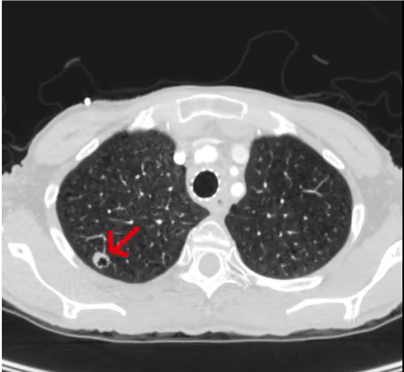
\includegraphics[width=5cm]{Images/ct-scan-orig.png} }}%
    \qquad
    \subfloat[Altered CT Scan]{{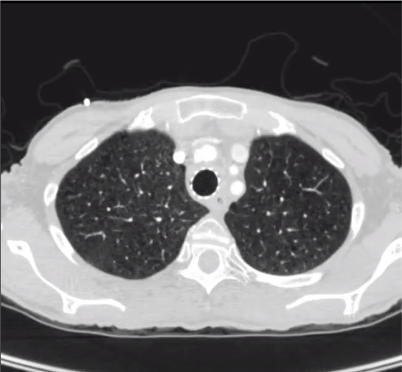
\includegraphics[width=5cm]{Images/ct-scan-alter.png} }}%
    \caption{Modification on CT Scans by Mirsky et al. \cite{mirsky_ct-gan_2019}}%
    \label{fig:example}%
\end{figure}
\addcontentsline{toc}{subsubsection}{Figure 1: Altered CT Scans} \\

By training a generative adversarial network on 888 CT scans, the images were successfully altered with deep learning. The effectiveness of the attack was then verified in a blind and open trial where radiologists were asked to diagnose complete CT scans. In general, the attack had an average success rate of 99.2\% for cancer insertion and a 95.8\% for cancer removal \cite{mirsky_ct-gan_2019}. This newfound application of malware places thousands of lives in danger and emphasizes the far-reaching repercussions of cyber attacks.

\subsection*{\color{SubSectionBlue}{Two Targets}}
\addcontentsline{toc}{subsection}{Two Targets} \\

When looking at the targets of these cyber attacks, there are two major firm-types present: bigger targets and small-medium targets. Bigger targets are firms that have a constant influx of money from the government and have substantial changes to their budget each year. Bigger targets can also include cybersecurity departments that receive a large portion of the firm’s budget and don’t have an immediate limit on monetary spending. On the other hand, small-medium targets, like their name suggests, are smaller firms that are heavily-restricted with the available funding for cyber security, generally working with a fixed budget \cite{fielder_decision_2016}. They can also include cybersecurity departments that receive a small portion of the firm’s budget and face immediate restrictions. This smaller budget forces trade-offs within the company where the chief technical officer has to make important decisions. The bigger targets have layers of security protecting the information making it more secure when compared to a smaller target that does not have the resources to implement that software. For this reason, approximately 72\% of cyber breaches occur at Small-Medium targets making the information more insecure when compared to bigger firms \cite{fielder_decision_2016}.  
\vspace{1mm}

However, smaller targets do provide substantial benefits to their customers despite their decrease in size. Due to the research and development nature of small-medium targets, they are likely to have more classified data when compared to bigger targets, who are trusted with more public data. On top of that, facilities like hospitals spend so much of their budget on equipment and staffing that little money gets allocated towards infrastructure development. The lack of funding increases the vulnerability of electronic health records. Since the data is more valuable, if there is a breach in a small-medium target, the risks are significantly higher when compared to a breach in a larger company. So, it is important for small-medium targets to implement controls that can mitigate vulnerabilities present in the system. Despite the importance of these controls, most Chief Information Security Officers (CISO) are not confident in patching up vulnerabilities under the budget constraint that is present in the company. For example, in a report published by Deloitte and NAISCO, 75.5\% of CISO’s cited a lack of sufficient budget as the top challenge (Fielder, 2016). Also, the study finds that 49\% of cybersecurity firms only have 6 to 15 specialists working to protect the data. 

\begin{figure}[ht]%
\centering
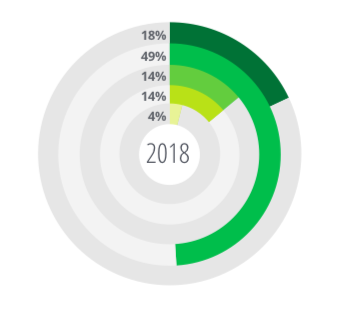
\includegraphics[width=5cm,height=5cm]{Images/expertise.png}
\caption{Top Restriction for Small Targets \cite{noauthor_deloitte_nodate}}%
\end{figure}
\addcontentsline{toc}{subsubsection}{Figure 2: Top Restriction for Small Targets} 

Each color in the chart [Fig 2] signifies a range of cybersecurity specialists . From the top (18\%) to the bottom (4\%), the first bar (18\%) represents 1-5 full-time employees, the second bar (49\%) represents 6-15 full-time employees, the third bar (14\%) represents 16-25 full-time employees, the fourth and last bar (4\%) represents 26-50 full-time employees. Since there is an abundant shortage of specialists in this field, action needs to be taken. For this reason, it is important to develop a system that will analyze the trade-offs of each control and advise the implementation of the controls that offer the greatest mitigation against an attack. 

\subsection*{\color{SubSectionBlue}{Endpoint Protection Data}}
\addcontentsline{toc}{subsection}{Endpoint Protection Data} \\

In an attempt to combat this growing issue, third-party organizations, like KnowBe4, publish statistics on the specifics of each attack in Endpoint Protection Reports. The Endpoint Protection Report provides information regarding the frequency of cyber attacks in a given year and the effectiveness of potential countermeasures which companies might implement to protect themselves. Using the 2009 endpoint protection report on security breaches and cost of downtime, Rakes et al. \cite{rakes_it_2012} from the Pamplin College of Business developed a dataset which consolidated the information in the report \cite{rakes_it_2012}. Qualitative attributes present in the endpoint protection report, such as countermeasure effectiveness, were expanded into quantitative values such as survival probabilities. The dataset expresses the relationships between a variety of different threats and countermeasures.

\begin{figure}[ht]%
\centering
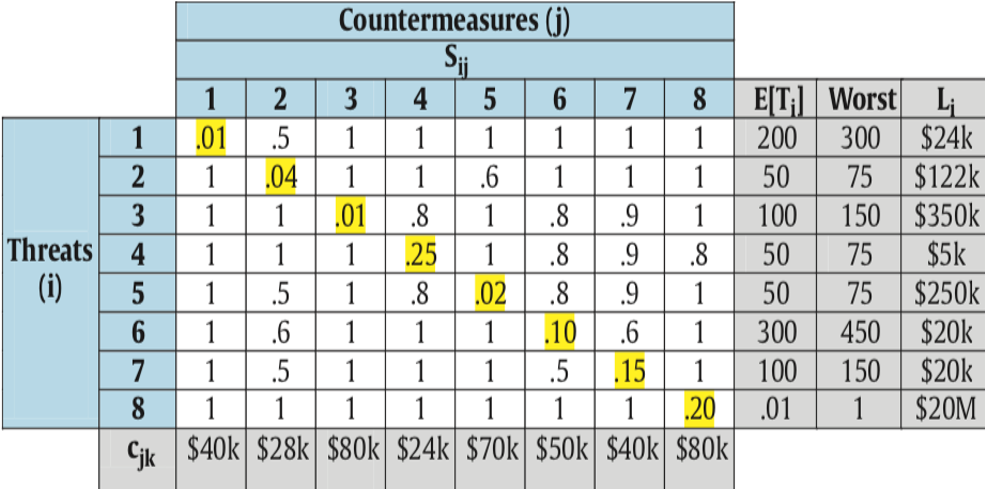
\includegraphics[width=15cm,height=5.15cm]{Images/protection-data.png}
\caption{Compiled Cybersecurity Data by Rakes et al. \cite{rakes_it_2012}}%
\end{figure}
\addcontentsline{toc}{subsubsection}{Figure 3: Compiled Cybersecurity Data} 

When analyzing the data set [Fig 3] compiled by Rakes et al. \cite{rakes_it_2012}, there are three major aspects that are taken into consideration: the survival probabilities, the general attack statistics, and the cost of implementing the countermeasures. The survival probabilities, which is the array in white, represent the probability, $P(X, Y)$, of an attack (X) succeeding when a certain countermeasure (Y) is implemented. Although all countermeasures are most effective against a specific threat, the array has off-diagonal terms because some countermeasures work not only against their primary threat, but because they provide additional protection against other threats as well. The general attack statistics, which are the three gray-shaded columns, represents the expected number of attacks in a given year ($E[T_i]$), the worst-case number of attacks in a given year ($W[T_i]$), and the damage incurred from each successful attack ($L_i$). Finally, the cost of implementing the countermeasures, the gray-shaded row, represents the monetary cost a company would have to pay in order to install that specific countermeasure. 

\subsection*{\color{SubSectionBlue}{Linear Optimization Model}}
\addcontentsline{toc}{subsection}{Linear Optimization Model} \\

Using this compiled data set, Rakes et al. \cite{rakes_it_2012} developed a linear optimization model that attempted to allocate budgets for companies of all sizes. The model selected countermeasures based upon quantitative factors such as threat levels and countermeasure effectiveness \cite{rakes_it_2012}.  The model took in the budget of a company as the input and attempted to choose appropriate countermeasures to protect that firm. Depending on the countermeasures chosen, the model would output the expected damage to the company in the case of an attack. In order to simulate the decision making process of firms, Rakes et al. followed three major steps. The first involved determining the probability $P_i$ that a threat $i$ would cause monetary loss.

\begin{equation}
P_i = \prod(1 - Y_i e_{ij}) 
\end{equation}

However, in order to linearize the model, the effectiveness, $e_{ij}$, was replaced with the proportion of threats that will survive an attack. On top of that, constraints were added to ensure that the proportion of threats which survived the first countermeasure would be assigned to the second countermeasure (Rakes, 2010). The process repeated for all countermeasures in which the binary selector, $Y_i$, was true. After the assignment process, the model estimated the damage to a company by surviving threats. The monetary loss (both explicit and implicit) was calculated by multiplying the number of surviving attacks by the loss per successful attack. This allowed Rakes et al. to approximate the amount of money saved by implementing each countermeasure. Once calculating the monetary loss, the model ensured that the cost of implementing the countermeasures would remain under a specified budget. 
\vspace{1mm}

Using the compiled data set [Fig 3], Rakes et al. \cite{rakes_it_2012} tested their linear optimization model on both the expected-case attacks and the worst-case attacks. The researchers looked at the relationship between company budget and monetary loss in the case of an attack. The loss was used as an indirect measure of the algorithm’s decision making capabilities. The monetary loss was predicted at each of 16 different budgets, comprising bigger and small-medium targets \cite{rakes_it_2012}.

\begin{figure}[ht]%
\centering
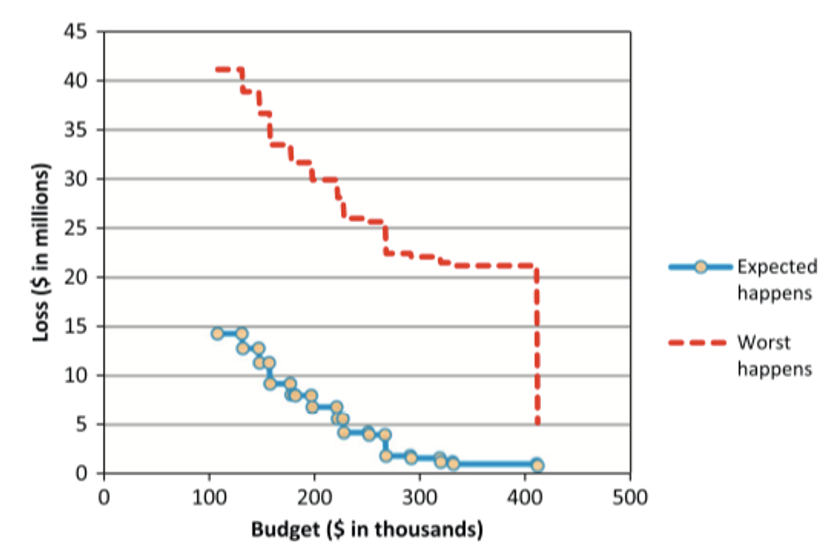
\includegraphics[width=9cm,height=6.5cm]{Images/linear-optimization.png}
\caption{Model Allocation at Each Budget Range \cite{rakes_it_2012}}%
\end{figure}
\addcontentsline{toc}{subsubsection}{Figure 4: Model Results}

When analyzing both the expected-case relationships and worst-case relationships of the linear model [Fig. 4], the budget and monetary loss seem to have an inverse relationship. With a higher budget, the algorithm can implement more countermeasures and the monetary loss faced by the companies is reduced. However, with small-medium targets, the linear optimization model predicts a high monetary loss in the case of an attack. So, an algorithm is needed that can help small-medium targets effectively allocate their cybersecurity budgets since it is these smaller targets that are more susceptible to malware.

\subsection*{\color{SubSectionBlue}{Knapsack Problem}}
\addcontentsline{toc}{subsection}{Knapsack Problem} \\

To improve the budget allocation of small-medium targets, the budget allocation problem has to be analyzed from a different angle. In fact, the complex trade-offs caused by a budget constraint can be simplified to a single-choice Knapsack problem. The knapsack problem is a NP-Complete optimization problem with the goal of finding, in a set of items with given values and weights, the subset of items with the highest total value, under a weight restriction \cite{murawski_how_2016}.

\begin{figure}[ht]%
\centering
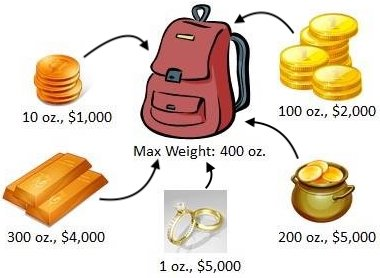
\includegraphics[width=5cm,height=5cm]{Images/knapsack-graphic.jpeg}
\caption{Knapsack Problem \cite{pan_comparison_2018}}%
\end{figure}
\addcontentsline{toc}{subsubsection}{Figure 5: Problem Explanation}

In this problem, a value has to be optimized while remaining under a certain constraint. A common interpretation of the knapsack problem is to design a system that can handle a large influx of data while remaining under corporate budget. Other interpretations include determining which parts to purchase in order to increase the fuel efficiency of a car. In the case of cyber security budget allocation, the mitigation of an attack has to be maximized while remaining under the budget constraint provided to the cybersecurity department of the small-medium target. Computer scientists have successfully solved this Knapsack problem classically; however, the algorithms are generally slow and time-consuming. With quantum computers providing a drastic increase in computational ability, new approaches can be designed to take advantage of a quantum computer’s unique properties like superposition and entanglement.

\subsection*{\color{SubSectionBlue}{Quantum Systems}}
\addcontentsline{toc}{subsection}{Quantum Systems} \\

With the complexity of mathematical problems, quantum computing can be a solution to avoid long periods of computation. A quantum computer uses fundamental principles of quantum mechanics, including superposition and entanglement, to overcome the limitation of a two-state classical system. In a traditional computer, data is encoded in bits, 0 and 1, which represent the on and off positions of a transistor; however, a quantum computer uses quantum bits, or qubits, to represent a weighted probability of the two initial states. Each qubit is mathematically notated as a vector, with a horizontal component that represents the probability of being a 0 and a vertical component that represents the probability of being a 1. The horizontal component will be referred to as $\alpha$, and the vertical component will be referred to as $\beta$. Although it is impossible to determine the exact state of a qubit, due to uncertainty and superposition, vector notation allows scientists to approximate this value using the direction and magnitude of the qubit. In a quantum system, or a space with multiple qubits, a major characteristic is that the magnitude of all of the probability vectors in the system must equal 1.
\vspace{1mm}

Another important aspect of any quantum system is the idea of measurement, which allows for a transformation of quantum states into classical states. A quantum entity, or system, only comes into existence and acquires definite properties when an observation or measurement is made \cite{forrester_quantum_nodate}. An important part of quantum mechanics are wave functions which give the mathematical probabilities of the state of a quantum entity before an observation has made \cite{forrester_quantum_nodate}. Each possible probability in the wave function is commonly referred to as an Eigenfunction. 

\begin{figure}[ht]%
\centering
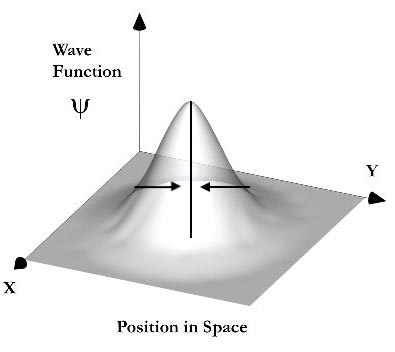
\includegraphics[width=5cm,height=5cm]{Images/eigen-function.jpg}
\caption{Quantum Measurement \cite{noauthor_copenhagen_nodate}}%
\end{figure}
\addcontentsline{toc}{subsubsection}{Figure 6: Quantum Measurement}

In order to obtain a measurable value from the system, the wave function must be collapsed into a specific Eigen function, as can be seen in Figure 6. In quantum mechanics, the possibilities of a wave function are localized into a single particle by adding energy and this localization results in measurement. However, the results from a measurement of the wave function is not random; every Eigen function has a certain probability of occurring. For quantum computing, there is a certain probability of returning 0 and a certain probability of returning 1.

\subsection*{\color{SubSectionBlue}{Quantum Genetic Algorithms}}
\addcontentsline{toc}{subsection}{Quantum Genetic Algorithms} \\

A possible application of quantum computing involves a quantum-genetic algorithm. A standard genetic algorithm is a population-based method which consists of 5 crucial components: initialization of a population, evaluation, parent selection mechanism, variation operators, and survivor selection \cite{garg_vector_2017}. 

\begin{algorithm}
\caption{Standard Genetic Algorithm}
\begin{algorithmic}[1]
\State $t \gets 0$
\State $f(x) \gets \text{Evaluation function}$
\State $population \gets \text{Initial Population}$
\While{$generation < \text{final generation}$}
        \State $values \gets f(population\text)$
        \State $survivors \gets \text{max(}values\text{)}$
        \For{$individual \in survivors$}
            \State $\text{Mutate the Survivors}$
            \State $population \gets \text{Survivor Offsprings}$
        \EndFor
        \State $generation += 1$
\EndWhile
\end{algorithmic}
\end{algorithm}

\addcontentsline{toc}{subsubsection}{Algorithm 1: Standard Genetic Algorithm}

Throughout the course of Algorithm 1, the population should “evolve'' towards an optimal solution. Although genetic algorithms are a good way to optimize problems, classical computers require additional steps in order to mutate the population. Genetic operators such as crossover probability and mutation effects have to be explicitly defined for the population to mutate. On top of that, these genetic operators require hyper parameter turning and will not accurately represent the random variability in most populations. 

\vspace{1mm}

When applied to quantum mechanics, however, previous research has indicated that a quantum genetic algorithm can be used based upon the concepts of quantum bits and quantum superposition states. Using qubit encoding, where each qubit uses a vector to represent binary code, a quantum algorithm can use a quantum system with multiple qubit vectors as an initial population \cite{wu_improvement_2013}. Specifically, each quantum gene is represented by a qubit vector, each quantum chromosome is represented by a bra vector, and each quantum population is represented by a column of chromosomes. When the quantum population is first created, each vector is initialized with a linear superposition of states, essentially setting both $\alpha$ and $\beta$ to  $\sqrt{2} / 2$ , so that the probability of getting a 0 or a 1 during measurement is the same.

\vspace{1mm}

Once the initialization of the population has been completed, the entire quantum population is measured. Measurement involves the evaluation of each individual in the population, as explained in Algorithm 1. However, the evaluation function will differ tremendously depending on the application of the quantum genetic algorithm. The qubit string which produces the highest profit while remaining under the constricting value is stored as the best individual in that generation. The fitness of the best population is then plotted on a curve for future use. In order to create a new generation from the existing quantum population, each qubit’s probability amplitudes are manipulated by a constant (a hyperparameter in the algorithm). When a new generation is created, the inherent randomness of quantum computing is utilized since this randomness creates natural variability in the population. The population will eventually reach a local maximum and the evolutionary algorithm is terminated \cite{nowotniak_higher-order_2014}. Thus, the theory of the genetic algorithm remains the same but a QIGA manipulates qubit vectors, instead of classical values, to create increase optimization.  Higher-Order quantum genetic algorithms use quantum registers to handle the encoding instead of isolated qubit vectors \cite{nowotniak_higher-order_2014}.

\subsection*{\color{SubSectionBlue}{Disaster Algorithm}}
\addcontentsline{toc}{subsection}{Disaster Algorithm} \\

The current setup of the quantum genetic algorithm does not account for the stabilization that occurs when an environment reaches a local optimum. A local optimum is when the genetic algorithm prematurely converges onto a single value for a certain period of time giving the illusion that the absolute maxima, or extremity point has been determined \cite{nowotniak_higher-order_2014}. So, one caveat of the genetic algorithm is the time of convergence in later states of the algorithm. 

\vspace{1mm}

Fu et al. \cite{wu_improvement_2013} addressed this issue and improved local search performance by implementing a self-adaptive rotating angle strategy and a disaster algorithm \cite{wu_improvement_2013}.  The rotating strategy exploited different concepts of linear algebra to decrease the number of parents with each call of the algorithm. The disaster condition, however, imposed a self-made disaster once the genetic algorithm reached a premature convergence value. For example, in some functions, there are various relative maxima and the genetic algorithm might mistake a relative maximum for an absolute maximum. In a quantum system, the disaster was usually resetting the probability amplitudes of some vectors to a linear superposition of states. This prevents premature convergence and ensures that the highest value for the knapsack function is returned.

\vspace{1mm}

Although Fu et al. \cite{wu_improvement_2013} did not test their algorithm using the knapsack problem, their method required similar computational abilities. After testing, researchers concluded that the addition of the rotating technique and the disaster condition improved the times of convergence of the quantum-inspired genetic algorithm, and returned a higher optimization value \cite{wu_improvement_2013}. However, the research that was performed by this team used isolated qubit vectors to encode qubit strings, as common with QIGA algorithms, and the simplicity of the design could have caused a lower optimization value than initially expected.

\subsection*{\color{SubSectionBlue}{Uniqueness of This Researcher's Current Work}}
\addcontentsline{toc}{subsection}{Uniqueness of This Researcher's Current Work} \\

The new research performed addresses the flaws in previous research and allows for greater theoretical optimization of the knapsack problem. In this new algorithm, Quantum Save, the higher-order quantum genetic algorithm is implemented on the IBM Q32 simulator which allows the algorithm to better simulate a quantum state. Quantum Save uses the increased complexity of the Q32 simulator to better mimic the random variations that occur in a genetic algorithm. In addition to that, although Kucharski and Nowotniak \cite{nowotniak_higher-order_2014} provided a range for the amount of probability amplitude manipulation, they didn’t provide a certain value. So, Quantum Save will consist of tuned hyper parameters for which the optimization of the Knapsack problem is the greatest. Also, with Quantum Save, a disaster condition will be added to the higher-order QGA to prevent premature convergence. In fact, social disasters technique, which applies a catastrophic operator once a local maximum is reached is one of the best methods to obtain the global extremity point instead of the local maxima \cite{rocha_preventing_1999}. In Quantum save, the disaster condition will implement a simple quantum catastrophe operator. Therefore, by tuning the higher-ordered QIGA, the probability of reaching a global maximum will increase drastically, and the optimization value for the knapsack problem will be much higher.

In addition to that, Quantum Save can help hospitals and defense contractors save millions by allocating the budgets of small and medium sized targets. In previous research, the cyber security investment model was based upon simulated values and game theory. And with the existing optimization models, like the one proposed by Rakes et al. \cite{rakes_it_2012}, the model performs significantly better for bigger targets since there is more budget to work with. The model does not face the full effect of the budget constraint and can easily choose countermeasures to maximize mitigation. However, it is the smaller-medium sized targets who are the most vulnerable to malware from adversaries. So, Quantum Save uses threat factors and mitigation values from real-life case studies to improve the budget allocation of these small-medium sized targets. Specifically, the data set compiled by Rakes et al. \cite{rakes_it_2012} in Figure 3 is inputted into the quantum algorithm. Researching this topic will allow the scientific and engineering community to accomplish countless tasks that have a limitation factor and an optimization value. Quantum Save can also improve the cybersecurity defenses of hospitals and defense contractors. \\


\section*{\color{SectionBlue}{Experimental Design}} \label{sec:sections}
\addcontentsline{toc}{section}{Experimental Design}
\subsection*{\color{SubSectionBlue}{Variables}}
\addcontentsline{toc}{subsection}{Variables} \\
In this research problem, the extent to which Quantum Save can optimize the spending of a cybersecurity budget is investigated. Using the data set defined by Rakes et al. \cite{rakes_it_2012}, Quantum Save will be implemented and an optimal investment strategy can be determined. The project will consist of two phases where the first phase involves tuning the Quantum Save algorithm with the optimal probability amplitude manipulation and implementation of the disaster algorithm. In this phase, it was hypothesized that the probability amplitude manipulation along with the disaster algorithm implemented on a POWER 9 architecture would result in the optimization of the Knapsack problem. For the first phase, the independent variable is the manipulation of the probability amplitudes and the implementation of the disaster algorithm while the dependent variable is the optimization of the Knapsack problem.

\vspace{1mm}

The second phase of the project involves applying the Quantum Save algorithm to the cyber security modeled previously defined and see if this algorithm can provide an optimal investment strategy for CISO’s. In this phase, it was hypothesized that if the Quantum Save algorithm is implemented in the cyber security investment problem, then the investment strategy that is obtained will be better when compared to previous case studies (specifically, the linear optimization model by Rakes et al. \cite{rakes_it_2012}). This is because Quantum Save has a better optimization of the knapsack problem when compared to that of previous research. Also, quantum computing would allow for a better simulation of random variability in the genetic algorithm. In this phase, the independent variable is the implementation of the QIGA algorithm with a cyber security purpose while the dependent variable is the investment strategy that is obtained after implementing the QIGA algorithm.

\vspace{1mm}

Quantum Save consists of six major steps and these individual steps are performed multiple times throughout the evolution process. Every time these steps are performed is called a generation and through multiple generations, the population should evolve to produce a greater optimization of the knapsack function. The steps in each generation derive from Darwin’s theory of evolution which states that evolution is a cause of overpopulation, competition between individuals of the species, and eventual survival of the fittest. However, before implementing the QIGA-2 algorithm on the IBM Q32 computer, various libraries including Qiskit by IBM and NumPy must be imported in order to connect with the quantum computer.

\subsection*{\color{SubSectionBlue}{Phase 1 of Quantum Save}}
\addcontentsline{toc}{subsection}{Phase 1 of Quantum Save} \\

The first section of the quantum genetic algorithm is reliant on the idea of over- population and natural variability in genes. As Darwin concluded, evolution is spurred when there are too few resources for too many individuals and random variability in the population cause some individuals to be better than others. In the first step, the quantum population is created and initialized. In this case, the population is an array of 32 qubits, the maximum number of qubits available on the IBM Q32, and each quantum chromosome represents a row in that array.

\begin{algorithm}
\caption{Quantum Save -- Phase 1}
\begin{algorithmic}[1]
\State $n \gets \text{number of countermeasures}$
\State $b \gets \text{budget}$
\State $probabilityAmplitude \gets [0.5, 0.5, 0.5, 0.5]$
\State $generation \gets 0$
\While{$generation < \text{10}$}
        \State $quantumRegister \gets 0$
        \While{$quantumRegister < \text{n}$}
            \State $classicalRegister \gets \text{classicalRegister[n]}$
            \State $quantumCircuit \gets \text{classicalRegister} + \text{quantumRegister}$
            \State $quantumCircuit \gets \text{probabilityAmplitude}$
            \State $job \gets measure(quantumCircuit)$
        \EndWhile
        \State $quantumRegister ++$
\EndWhile
\end{algorithmic}
\end{algorithm}
\addcontentsline{toc}{subsubsection}{Algorithm 2: The First Phase} 

The array of 32 qubits is arranged to simulate a Think-Tank of four Chief Security officers. The goal of the Think Tank is to create a recommendation list of 8 countermeasures which defense contractors and small-medium targets across the world can implement in order to protect themselves from foreign attacks. Each of the four rows in the qubit array, or matrix, represents a Chief Security Officer in the think-tank, and each of the eight columns in the qubit array represents a countermeasure on the recommendation list. If the qubit returns a value of 1, then the countermeasure is added to the recommendation list. On the other hand, if the qubit returns a value of 0, then the countermeasure is removed from the recommendation list (Fig. 7). 

\begin{figure}[ht]%
\centering
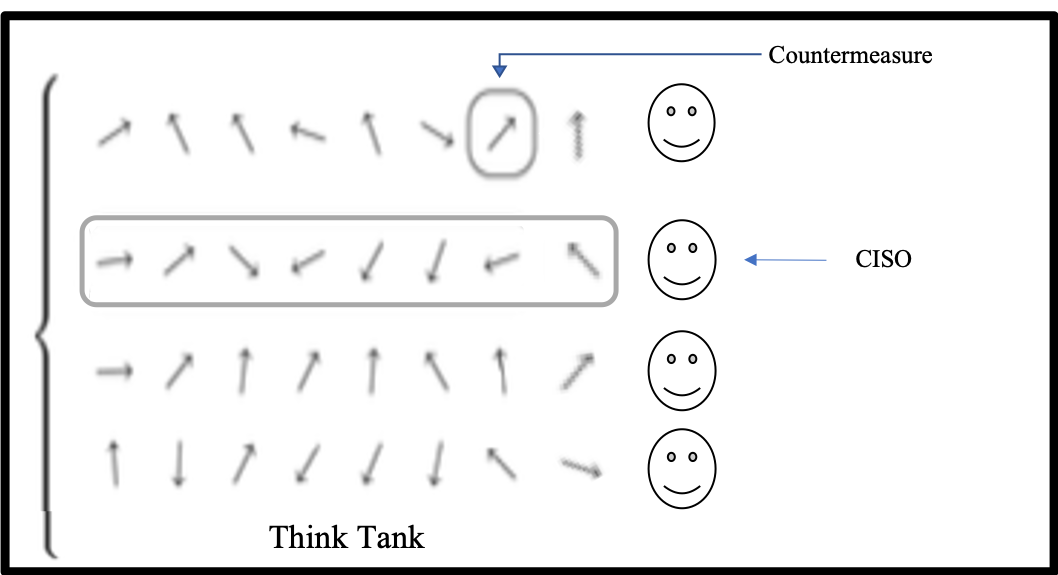
\includegraphics[width=10cm,height=5cm]{Images/quantum-population.png}
\caption{Quantum Population on Q32}%
\end{figure}
\addcontentsline{toc}{subsubsection}{Figure 7: Quantum Population on Q32} 


\vspace{1mm}

After the quantum population is created, each qubit register in that population is initialized with a linear superposition of states. By starting out with an equal chance of getting one and zero, there is natural variability in the population and the genetic algorithm can be more effective. In the case of the cyber security application, the linear superposition of states that the quantum population is initialized with represents an equal probability of a defender implementing a certain control and not implementing that control. Therefore, there is natural variability in the population and the genetic algorithm is effective.

\subsection*{\color{SubSectionBlue}{Phase 2 of Quantum Save}}
\addcontentsline{toc}{subsection}{Phase 2 of Quantum Save} \\

Now that the population has been created and has been initialized with a linear superposition, the second section of the quantum genetic algorithm can begin. This section the individuals with the best random attributes are chosen and the fittest individuals in the population, or those who pack the knapsack the best, will remain for the next generation. After the initialization of the quantum population, it will be classically measured by collapsing the existing wave function. Depending on the alpha and beta values present in each qubit register, a binary string of size two, either 00, 01, 10 or 11, will be obtained from each register 

\begin{algorithm}
\caption{Quantum Save -- Phase 2}
\begin{algorithmic}[1]
\State $CISO \gets 0$
\While{$CISO < \text{4}$}
        \State $binaryString \gets \text{""}$
        \State $result \gets \text{""}$
        \While{$result \text{ in job}$}
            \State $binaryString \gets binaryString + \text{Most Frequent String}$
        \EndWhile
        
        \State $countermeasure \gets 0$
        \State $knapsack \gets 0$
        \While{$countermeasure \text{ in binaryString}$}
            \State $knapsack \gets knapsack + countermeasure$
            \If{$knapsack > b$}
                \State $knapsack \gets knapsack - countermeasure$
            \EndIf
            \State $profit \gets \text{amount saved[}countermeasure\text{]}$
        \EndWhile
        \State $bestIndividual \gets max(profit)$
\end{algorithmic}
\end{algorithm}
\addcontentsline{toc}{subsubsection}{Algorithm 3: The Second Phase} 

During each fitness evaluation, or the conversion between quantum and classical states, the qubit register is measured 1024 times and the most consistent binary string is returned. The binary strings from every four registers will then be combined until four classical strings are obtained, one for each individual in the Think Tank. 

\vspace{1mm}

After quantum measurement, using the Copenhagen interpretation, is complete, the binary strings are evaluated in order to determine the best individual. Depending on the binary string, which essentially represents the controls that are implemented by the defender, a certain mitigation will be received. In this case, if there is a 1 that means that the defender chose to implement a specific control. On the other hand, if there is a zero, then the defender didn’t implement a certain control. Apart from the profit value, a total weight for the knapsack was also obtained, or the total cost of implementing all of the controls, and that total cost was compared to the cost cap, or the budget, set before the first generation. After each binary string is evaluated, the binary string, and respective individual, with the highest profit value is stored as the best chromosome. With the application to a cyber security investment problem, the best chromosome will be the defender that implemented the controls that resulted in the greatest mitigation of the attack.

\subsection*{\color{SubSectionBlue}{Phase 3 of Quantum Save}}
\addcontentsline{toc}{subsection}{Phase 3 of Quantum Save} \\

Since the best strategy to mitigate an attack on the defender’s small-medium enterprise has been determined, the probability amplitudes of each qubit register will be manipulated in the following manner.

\begin{algorithm}
\caption{Quantum Save -- Phase 3}
\begin{algorithmic}[1]
\State $binaryArray \gets binaryString.split()$
\State $CISO \gets 0$
\While{$CISO < 4$}
    \State $countermeasure \gets 0$
    \While{$countermeasure \text{ in } binaryArray$}
        \If{countermeasure != bestIndividual}
            \State $probabilityAmplitude \gets \text{manipulate[}probabilityAmplitude\text{]}$
        \EndIf
        \State $probabilityAmplitude \gets probabilityAmplitude$
    \EndWhile
\EndWhile
\end{algorithmic}
\end{algorithm}
\addcontentsline{toc}{subsubsection}{Algorithm 4: The Third Phase} 

Initially, the first binary pair in the best individual will be obtained and depending on the value of that pair, the probability distribution will be normalized to one. On the other hand, all of the other probability amplitudes will decrease by a factor of $probabilityAmplitude$, a hyper parameter in the algorithm. In this case, the probability of a defender implementing the successful controls increases while the probability of a defender implementing the unsuccessful controls decreases. The factor of probability manipulation, $probabilityAmplitude$, is a hyper parameter of this algorithm and this hyper parameter was tuned by testing out different values for and observing the optimization of the knapsack problem. In the end, the controls that resulted in higher mitigation of an attack were encouraged while controls that resulted in lower mitigation of an attack were discouraged (Fig 8).

\begin{figure}[ht]%
\centering
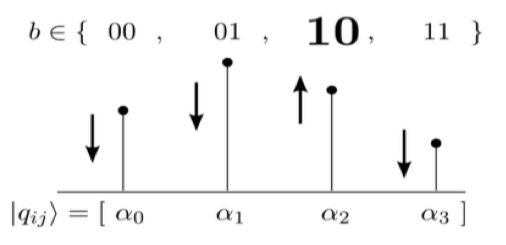
\includegraphics[width=10cm,height=5cm]{Images/amplitude-man.png}
\caption{Manipulation of Probability Amplitudes}%
\end{figure}
\addcontentsline{toc}{subsubsection}{Figure 8: Manipulation of Probability Amplitudes} 

At this point, the algorithm has completed one generation of fitness evaluations. In order to obtain an accurate optimization of the knapsack problem, this process needs to be repeated for 10 generations in order to get a higher optimization of the knapsack problem. At the end of these ten generations, the data of final profit outputted by Quantum Save will be obtained and that data can be compared to that of previous research. However, now that the probability amplitude manipulation is complete and the optimal value has been determined, a disaster algorithm will be implemented. In this case, the disaster algorithm will simply reset the population to a linear superposition of states in the middle of Quantum Save. However, the generation that the disaster algorithm is implemented, is a hyper parameter of this algorithm and this hyper parameter was tuned by testing out different generations. In the end, the location of the disaster algorithm was chosen by the overall mitigation of an attack by the defender.

\vspace{1mm}

After one instance of the algorithm, or 10 generations, has completed its run-time, the data of final profit outputted by Quantum Save will be obtained and that data will be compared to that of previous research. On top of that, the different hyper parameters including the value and the generation for the disaster algorithm will be tuned.

\subsection*{\color{SubSectionBlue}{Why Quantum Computing}}
\addcontentsline{toc}{subsection}{Why Quantum Computing} \\

With this quantum algorithm, one important aspect is the evolution of the population. In order for a population to evolve, there needs to be random variation in the population so that certain traits emerge over others. If every generation contained the same traits, then the entire population would either die or survive. Instead, mutations and gene crossovers drive the idea behind natural selection. With this evolution process, a quantum computer would significantly enhance the effect of a genetic algorithm. \newpage

\begin{figure}[ht]%
    \centering
    \subfloat[General Qubit Properties]{{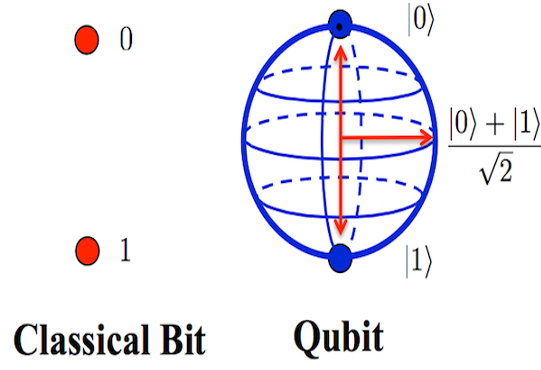
\includegraphics[width=6cm]{Images/qubit.png} }}%
    \qquad
    \subfloat[IBM Quantum Simulator]{{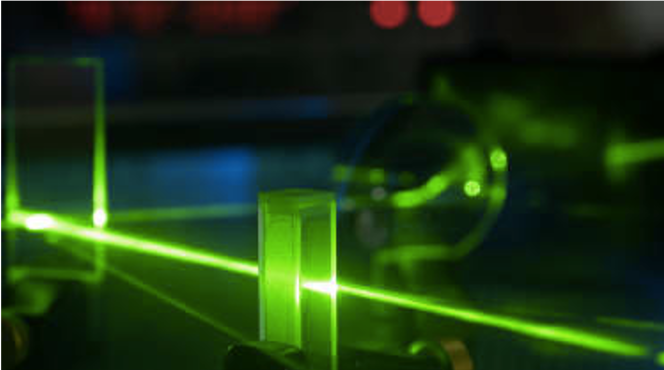
\includegraphics[width=5cm]{Images/ibm_q.png} }}%
    \caption{Power of the Qubit}%
    \label{fig:example}%
\end{figure}
\addcontentsline{toc}{subsubsection}{Figure 9: Power of the Qubit} \\

On a traditional classical computer, a bit is isolated to either 0 or 1, but a qubit uses quantum mechanical properties to simulate a weighted probability distribution between 0 and 1. Each qubit is initialized with a 50\% chance of returning 1 and a 50\% chance of returning 0. As the algorithm progresses, the probabilities change, with a potential 90\% chance of returning 1 and a 10\% chance of returning 0. In a classical genetic algorithm, random variation is controlled by unique constants. However, by using quantum computing, the random variation is inherent within the computational method. The measurement value of a qubit is never concrete but fluctuates based upon probability amplitudes. More specifically, the IBM quantum simulator uses a dilution refrigerator to suspend an electron and shoot a pulse at the suspended electron. If the electron is spin-up, the qubit returns a zero. On the other hand, if the electron is spin-down the qubit returns a one. This allows the IBM Q32 simulator to accurately simulate a quantum state.









\section*{\color{SectionBlue}{Results}} \label{sec:sections}
\addcontentsline{toc}{section}{Results}
\subsection*{\color{SubSectionBlue}{Tuning Hyperparameters}}
\addcontentsline{toc}{subsection}{Tuning Hyperparameters} \\

The first phase of data collection involves tuning the actual hyper parameters of the quantum genetic algorithm. One hyper parameter that needs to be tuned is the µ value that describes how much the probability amplitudes are manipulated when the quantum population is evolving. This hyper parameter is important because it is fundamental when describing the probability amplitude manipulation that occurs in each generation of the genetic algorithm. It helps determine which cyber security controls are optimal and successful in mitigating attacks.  Depending on the value for µ, the optimization of the knapsack problem can either increase or decrease. In this research, four different values for µ were tested including 0.8, 0.9, 0.95, and 0.99 and the final optimization of the knapsack problem was recorded. \\ \newpage

\vspace*{0.6cm}
\begin{table}[H]
    \centering
    \caption{Results of Quantum Save with Varying Hyperparameters}
    \label{parametri}
    \resizebox{0.85\textwidth}{!}{%
    \begin{tabular}{@{}1lllll1111@{}}
    \toprule \\
    
    
    \multicolumn{1}{c}{\textbf{Statistics}} &
    \multicolumn{5}{c}{\textbf{Probability Manipulation}} & \multicolumn{4}{c}{\textbf{Disaster Algorithm}} \\
    \cmidrule(r){1-1}   \cmidrule(lr){2-6} \cmidrule(lr){7-10} \\

    Trial & 80\% & 90\% & 95\% & 99\% & \textit{Baseline} & 5  & 6  & 7 & \textit{Baseline}  \\  \midrule
    1 &	8957 &	9528 &	9416 &	7004 & 5662 & 7503 & 7689 &	8853 & 9528 \\
    2 &	7509 &	7723 &	8039 &	5885 & 6406 & 7017 & 7117 &	8432  & 7723	\\
    3 &	8631 &	10436 &	7108 &	7261 & 6920 & 8642 & 7277 &	9290  & 10436 \\
    4 &	8005 &	9352  &	7040 &	6135 & 5980 & 9920 & 7793 &	9696 & 9352	 \\
    5 &	8149 &	7566 &	7462 &	8179  & 9678 & 8390 & 8398 & 8722 & 7566	\\
    6 &	8299 &	7324 &	6941 &	7030 & 8775 & 9323 & 8031 &	8154 & 7324	 \\
    7 & 7798 &	8368 &	9753 & 7076 & 9258 & 8762 & 8338 & 8459 & 8368	 \\
    8 &	9303 &	8504  &	7077  &	8418 & 7070 & 7945 & 8484 &	6486 & 8504	\\
    9 &	7799 &	6020  &	7161 &	8649 & 6954 & 7044 & 8232 &	7910 & 6020	 \\
    10 & 8230 & 7008 &	9684 &	9064 & 4097 & 8448 & 8008 &	7736 &  7008	\\
    AVG	& 8150 & 8252 & 7975 & 7641 & 7086 & 8518  & 8235 & 8292  & 8252 \\
    SE	& 156.51	& 310.67 & 266.80 &	293.33& 414.21  & 	236.19 & 241.81 & 214.09 & 310.67 \\     
    \bottomrule
    \end{tabular}}
\end{table}
\addcontentsline{toc}{subsubsection}{Table 1: Results of Quantum Save with Varying Hyperparameters} \\

{\footnotesize *** The first 10 trials out of 15 total are shown. All values are in dollars. The baseline for the Disaster Algorithm is Quantum Save's performance with simply probability amplitude manipulation. The baseline for the Probability Manipulation is Quantum Save's performance without the manipulation. \par}

\vspace{1mm}

These specific values were chosen for a reason when dealing with probability amplitude manipulation. At first, based upon patterns observed in Nowotniak and Kucharski's initial research \cite{nowotniak_higher-order_2014}, higher probability manipulation values, such as 99\% would be around the optimal manipulation value since that would drastically increase the probability of implementing a successful control. However, after running the algorithm under this high manipulation value, it was realized that an excessively high value would result in over fitting, where each defender was too reliant on the patterns of the best individual. So, the value was reduced to 80\%. After running the algorithm again, it was determined that the defenders in this generation are not as reliant on the patterns discovered in previous generations and a lower optimization was occurring. So, as a compromise, the value was raised to 95\% and then lowered back down to 90\% to get a variety of probability amplitude coefficients.

\vspace{1mm}

After this data was collected regarding the probability amplitude manipulation, another vital hyper parameter was the generation at which to implement the disaster algorithm. Depending on the generation that the disaster algorithm was implemented at, the optimization of the Knapsack problem and the choosing of countermeasures changed. For example, if the disaster algorithm was implemented towards the later generations, then the behaviors of the defenders would not impact the overall optimization of the Knapsack problem and the company would get stuck at the local maximum. On the other hand, if the disaster algorithm was implemented towards the earlier generations,t hen the company would not receive the higher level of mitigation that the previous generation had gotten. Either way, there is a trade-off between getting stuck at a local maxima and not even reaching that local maxima. To resolve this trade-off, it is important to tune the disaster algorithm hyper parameter as done in Table 1. The data collection started at a disaster step of 7 and then slowly decreased to 6 and eventually to 5. For each of these disaster steps, Quantum Save was run, with all 10 generations, and the final output was recorded.

\subsection*{\color{SubSectionBlue}{Cybersecurity Application}}
\addcontentsline{toc}{subsection}{Cybersecurity Application} \\

Now that the hyper parameters have been tuned, Quantum Save can be implemented in the context of a cyber security investment problem where a small-medium target has to implement controls that result in the highest mitigation. The total mitigation across 10 generations was recorded and Quantum Save was run 10 times in order to determine whether the mitigation is better than that of existing case studies, specifically the linear optimization model proposed by Rakes et al. \cite{rakes_it_2012}. 

\begin{singlespace}
\vspace*{0.6cm}
\begin{table}[H]
    \centering
    \caption{Quantum Save vs. Other Budget Allocation Models}
    \label{parametri}
    \resizebox{0.75\textwidth}{!}{%
    \begin{tabular}{@{}1lll@{}}
    \toprule
    Budget & Quantum Save & Linear Algorithm & Brute Force Algorithm \\ \midrule
    80k & 26.57 M & 32.20 M & 14.29 M \\
    108k & 14.26 M & 14.29 M & 11.24 M \\
    132k & 11.95 M & 12.78 M & 8.294 M \\
    148k & 11.31 M & 11.32 M & 5.244 M \\
    158k & 8.340 M & 9.184 M & 5.244 M \\
    178k & 7.714 M & 8.071 M & 5.244 M \\

    \bottomrule
    \end{tabular}}
\end{table}
\end{singlespace}
\addcontentsline{toc}{subsubsection}{Table 2: Quantum Save vs. Other Budget Allocation Models} \\

The data shows the relationship between the budget of the company and the monetary loss due to a cyber attack. The relationship between the two variables and the effectiveness of Quantum Save will be investigated later. Now that the data concerning Quantum Save's accuracy has been collected, the next step of the research centered around the run time of the algorithm. When analyzing an algorithm's effectiveness, the speed of the algorithm needs to be taken into account. More specifically, data was gathered surrounding Quantum Save's scalability, or how the size of the input (number of countermeasures in the recommendation list) affected the run time of the algorithm. The data collection process involved obtaining the run time of the algorithm across 10 trials for each permutation of input sizes. The run time was measured using the internal clock on both the quantum simulator and the classical machine. The input sizes varied anywhere from 1 countermeasure in the recommendation list to 8 countermeasures in the recommendation list. After collecting data about the scalability of Quantum Save, the same procedure was completed for the Brute Force algorithm for comparison purposes. 

\section*{\color{SectionBlue}{Analysis}} \label{sec:sections}
\addcontentsline{toc}{section}{Analysis}
\subsection*{\color{SubSectionBlue}{Hyperparameters}}
\addcontentsline{toc}{subsection}{Hyperparameters} \\

Throughout this research, there were two major changes that distinguished Quantum Save when compared to existing algorithms. The first is the utilization of quantum computing, or the IBM Q32 quantum simulator. To evaluate the effectiveness of quantum computing in optimizing the Knapsack problem, or more accurately the cybersecurity defense problem, the evolution of Quantum Save was compared to that of Kucharski and Nowotniak \cite{nowotniak_higher-order_2014}. 
Kucharski and Nowotniak \cite{nowotniak_higher-order_2014} used a classical implementation of the quantum-inspired genetic algorithm to find a solution to the knapsack problem.In order to establish the significance of Quantum Save in the context of the Knapsack problem, the baseline optimization that was obtained, without any probability amplitude manipulation, was compared to the highest value obtained by Nowotniak and Kucharski \cite{nowotniak_higher-order_2014}, \$5709.

\vspace{1mm}

In order to compare the results of Quantum Save when compared to previous research, a 1-sample t-test with a significance level of 0.05 was run on the baseline probability manipulation (Table 1) and the results of the test were used to determine whether Quantum Save on the IBM Q32 simulator was significantly better when compared to Kucharski and Nowotniak \cite{nowotniak_higher-order_2014}. Since both of the p-values (one-tailed and two-tailed) obtained from the 1-sample t-test, \textit{0.003} and \textit{0.005} respectively, were less than the established significance level of 0.05, the null hypothesis could be confidently rejected. If the null hypothesis was true, as the proposed algorithm didn’t perform any better than that of previous research, there would only be a 0.274 or 0.548 percent chance of obtaining a profit value this high or higher based upon random sampling variability alone. Therefore, there is enough statistical evidence to suggest that Quantum Save on the IBM Q32 computer performed significantly better than that of previous research. In the end, Quantum Save, on the IBM quantum simulators, likely performed better due to the simulation of more qubits and the existence of four quantum chromosomes in the population as opposed to three. These factors allowed for more genetic variability and increased the chance of finding the non-obvious solutions to the knapsack problem. Different routes were taken and ultimately, a higher optimization of the knapsack function was achieved. 

\vspace{1mm}

However, Quantum Save was improved by tuning hyper parameter values including the value of µ which described the amount of probability amplitude manipulation and the generation for which to implement the disaster algorithm. First, when regarding the manipulation of probability amplitudes, an analysis of variance test, or an ANOVA test, was run to determine whether the change in probability amplitudes did in fact achieve a statistically significant change in the optimization of the knapsack problem. The significance level of the ANOVA test was 0.10 and that represented the alpha power of this statistical test. When implementing the probability amplitude manipulation, the goal was to simply increase the optimization of the knapsack problem. So, the alpha power of the test did not need to be extremely high so a value of 0.1 was chosen. Since the p-value of \textit{.052} is less than the significance level of 0.1, the null hypothesis could be confidently rejected. If the null hypothesis was true, as the proposed algorithm with manipulation of amplitudes did not perform any better than the algorithm without the manipulation of amplitudes, there would only be a 5.27\% chance of obtaining a profit value this high or higher based upon random sampling variability alone. Therefore, there is enough statistical evidence, within the power of this ANOVA test, to suggest that the manipulation of probability amplitudes increased the optimization of the knapsack problem. Since the ANOVA test does not provide the greatest value for µ, that had to be calculated manually. When looking at the data table, it could be observed that a µ value of 0.9 or a 90\% manipulation of amplitudes resulted in the highest optimization of the knapsack problem. In order to confirm the values obtained from the ANOVA test, the maximum profit over the probability amplitudes were observed. 

\vspace{1mm}

The second tuned hyper parameter was the generation on which to implement the disaster algorithm. To determine whether the disaster algorithm achieved a statistically significant change in the optimization of the Knapsack problem, another analysis of variance test, or an ANOVA test, was run. Again, like with the manipulation of probability amplitudes, the the significance level of the ANOVA test was 0.10 and that represented the alpha power of this statistical test. With a p-value of \textit{0.848}, it appears that the disaster algorithm does not significantly increase the optimization of the Knapsack problem. However, in Table 1, a disaster step of 6 does increase the optimization of the knapsack problem by around 3.22\%. Although this is not statistically significant, there is some improvement. The disaster algorithm will help only when Quantum Save reaches a local maxima, which might not occur in every  trial. So, with any improvement, the disaster algorithm is considered successful. Also, when looking at Table 1, the standard error with the disaster algorithm is much lower when compared to the baseline. This suggests that the disaster algorithm is preventing Quantum Save from getting caught on the lower local maxima. Now, the probability of finding that non-obvious solution increases drastically. 

\subsection*{\color{SubSectionBlue}{Accuracy of Quantum Save}}
\addcontentsline{toc}{subsection}{Accuracy of Quantum Save} \\

The second uniqueness of Quantum Save when compared to previous research, such as the linear optimization model \cite{rakes_it_2012} is the implementation of the QGA algorithm in cybersecurity budget allocation. However, when analyzing the effectiveness of Quantum Save in the realm of cybersecurity budget allocation, there are two distinct features that need to be considered: the accuracy and the run time. With the accuracy, the budget allocation techniques of Quantum Save can be compared with the techniques from linear optimization models \cite{rakes_it_2012}. The techniques will be quantified by analyzing the amount of money that a small-medium target will lose when implementing the countermeasures suggesting by each respective algorithm. The better algorithm will be the one that results in lower monetary loss in the case of an attack by foreign or domestic adversaries. From a simple eye-test on the data presented in Table 2, it appeared that my algorithm performed better when compared to previous research \cite{rakes_it_2012} at every budget range. However, the extent of that improvement varied significantly (Table 3).

\begin{singlespace}
\vspace*{0.6cm}
\begin{table}[H]
    \centering
    \caption{Percent Improvement by Quantum Save}
    \label{parametri}
    \resizebox{0.27\textwidth}{!}{%
    \begin{tabular}{@{}1l@{}}
    \toprule
    Budget & \% Improvement \\ \midrule
    80k & 17.48 \\
    108k & 0.24 \\
    132k & 6.53 \\
    148k & 0.05 \\
    158k & 9.19 \\
    178k & 4.42 \\
    \bottomrule
    \end{tabular}}
\end{table}
\end{singlespace}
\addcontentsline{toc}{subsubsection}{Table 3: Percent Improvement by Quantum Save} \\

When looking at Table 3, it was determined that Quantum Save performed better when compared to the generalized linear optimization model. But, the extent of that improvement varied from 0.05\% to 17.48\%. Since the discrepancy in the percent improvement is so high, another statistical method had to be taken to ensure that the improvement was not caused by random variability. The distribution of Quantum Save's outputs at each budget range was analyzed using a box plot (Figure 10).

\begin{figure}[ht]%
\centering
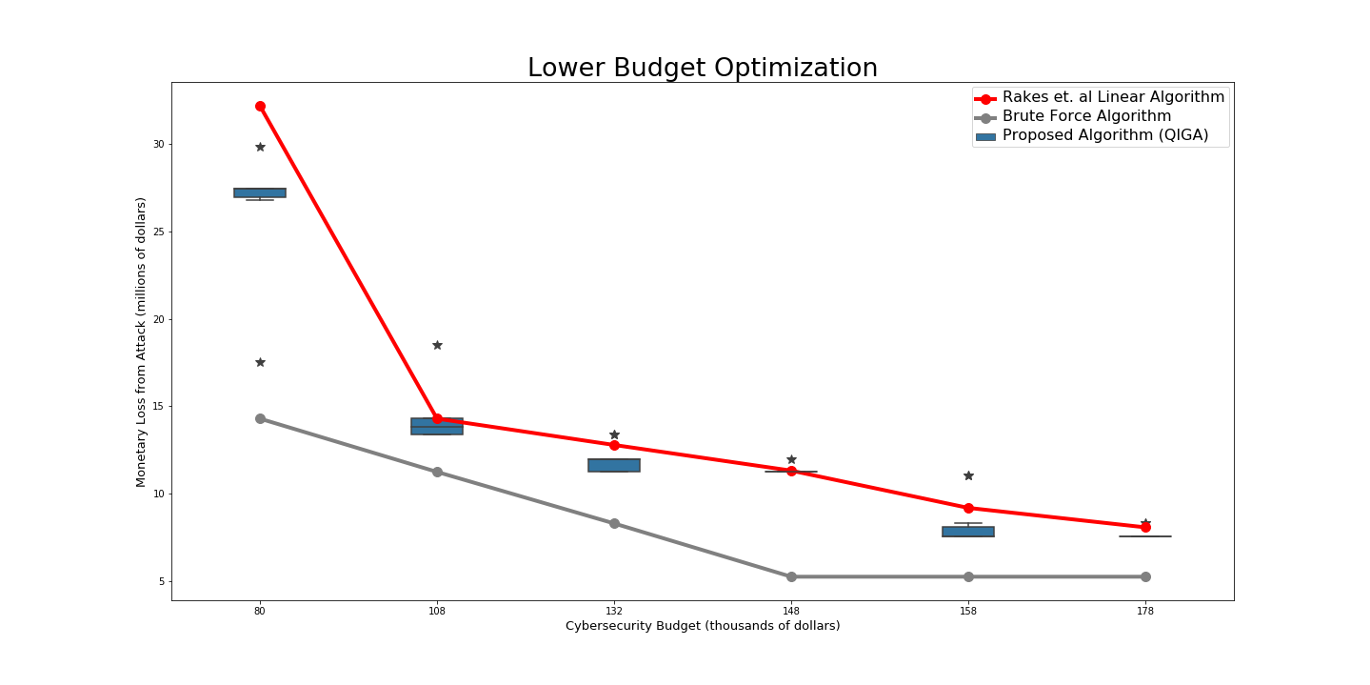
\includegraphics[width=11cm,height=5.6cm]{Images/boxplot.png}
\caption{Distribution of Quantum Save's Results by Budget}%
\end{figure}
\addcontentsline{toc}{subsubsection}{Figure 10: Distribution of Quantum Save's Results by Budget} 

When analyzing the box plot, data points that were outside of a standard 95\% confidence interval, or a 1.57 IQR range were labeled as outliers (as can be seen by the stars on the box plot). So, based upon the distribution of outputs shown in the box plot, barring outliers, it appears as if Quantum Save's results for the expected-case number of attacks per year were either less than or equal to the linear optimization mode. \cite{rakes_it_2012}. Although in some budgets Quantum Save allocated budgets as effectively as the linear model, that still serves to emphasize the significance of Quantum Save in the realm of allocating cybersecurity budgets. 

\subsection*{\color{SubSectionBlue}{Time Complexity of Quantum Save}}
\addcontentsline{toc}{subsection}{Time Complexity of Quantum Save} \\

The second technique for analyzing the uniqueness in Quantum Save when compared to previous research, such as the linear optimization model proposed by Rakes et al. \cite{rakes_it_2012}. In typical countermeasure recommendation lists, there are approximately 50 to a 100 countermeasures meaning any algorithm that attempts to allocate cybersecurity budgets needs to scale well. Using an algorithm which scales exponentially would be extremely time consuming, which is a luxury that most smaller-medium targets can not afford. Instead, a cybersecurity budget allocation algorithm needs to be able to produce high number countermeasure recommendation lists in a reasonable amount of time. To ensure that Quantum Save could meet that criteria, the run time of the algorithm was measured. The data was then analyzed by finding both an experimental and theoretical relationship between the number of countermeasures in the recommendation list and the run time of the algorithm. When considering experimental data, the run time of both a traditional brute force algorithm and Quantum Save was charted. Brute force was chosen as a comparison algorithm because it has the best accuracy of any potential cybersecurity budget allocation problem. 

\begin{figure}[ht]%
    \centering
    \subfloat[Quantum Save Time Complexity]{{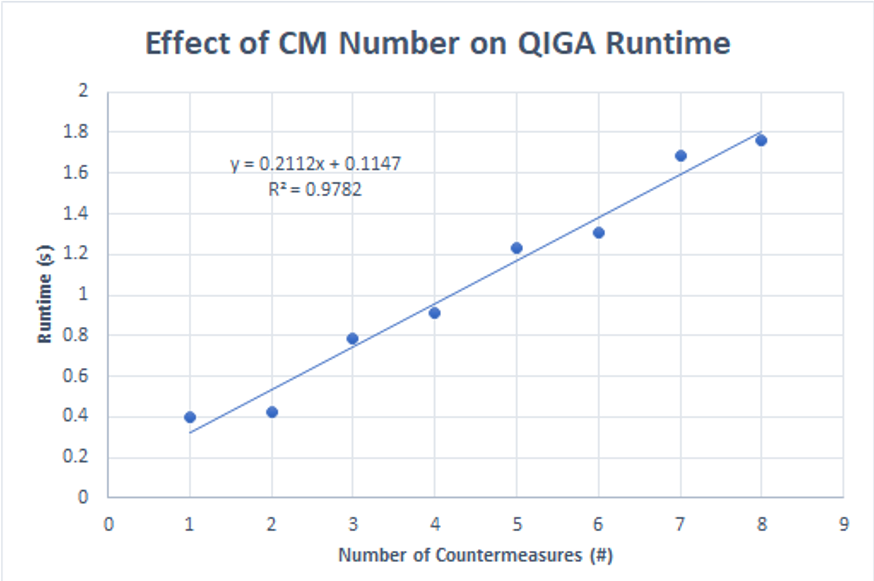
\includegraphics[width=7.65cm]{Images/q-save-runtime.png} }}%
    \qquad
    \subfloat[Brute Force Time Complexity]{{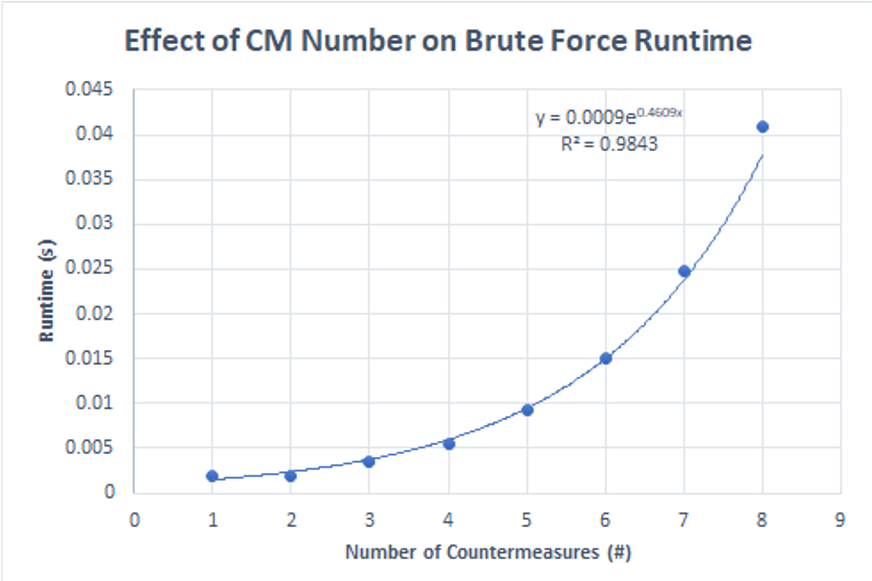
\includegraphics[width=7.65cm]{Images/brute-force-runtime.png} }}%
    \caption{Time Complexity of Quantum Save vs. Brute Force}%
    \label{fig:example}%
\end{figure}
\addcontentsline{toc}{subsubsection}{Figure 11: Time Complexity of Quantum Save vs. Brute Force} \\

The run time results, which showed the relationship between the run time of a Brute Force algorithm and the size of the input, was fitted with an exponential trend line and an r-squared value of 0.9843 was obtained. This high r-squared value suggests that 98.43\% of the variation in the run time of the algorithm was explained by the difference in input size, or the difference in the size of the countermeasure recommendation lists. The experimental results makes sense since Brute Force algorithms generally scale exponentially. This replication of Brute Force scalability provides justification for using this experimental method of determining run time. The other pair of results results, which showed the relationship between Quantum Save's run time and the size of the input, was fitted with a linear trend line and an r-squared value of 0.9782 was obtained. Again, this high r-squared value suggests that 97.82\% of the variation in the run time of the algorithm was explained by the difference in input size, or the difference in the size of the countermeasure recommendation lists. This experimental data provides an initial suggestion that the algorithm scales linearly, but a theoretical justification is needed to supplement the idea. 

\begin{lemma}
Quantum Save can allocate budget, $b$, when choosing from countermeasures with input-size, $n$, in $\mathcal{O}(n)$ time complexity with oracles for quantum measurement of a single register.
\end{lemma}

\begin{proof}
In the first line of Algorithm 2, the first phase of Quantum Save, the number of countermeasures is defined. This definition directly depends upon the input-size of the recommendation list, resulting in a complexity of $\mathcal{O}(n)$. From lines 2 - 4, basic variables for Quantum Save are defined. Since these variables are not correlated to the input-size, the resulting complexity is $\mathcal{O}(1)$. In line 5 - 6, the first loop begins which loops through the number of generations and the quantum register variable gets initialized. Again, since the number of generations is not correlated to the input-size, the resulting complexity of these lines is $\mathcal{O}(1)$. In line 7, a second loop begins which loops through every quantum register in the population. Since the quantum registers depend on the input size, these lines have a complexity of $\mathcal{O}(n)$. In lines 8 - 11, the quantum circuit is created and measured. Since the measurement of a single register does not depend on the size of the input, these lines have a complexity of $\mathcal{O}(1)$. Because the highest complexity is $\mathcal{O}(n)$ and there are no nested loops of higher complexity, the complexity of the first phase is $\mathcal{O}(n)$.

\vspace{1mm}

In the first two lines of Algorithm 3, the second phase of Quantum Save, the CISO variable is initialized and all of the CISO's are looped through. Since the number of CISO's does not vary based upon input size, the complexity of these lines is $\mathcal{O}(1)$. After a couple of definitions, which are $\mathcal{O}(1)$, the results of the quantum measurement are looped through in line 5. Since the job string would be longer if there are more countermeasures in the input, the complexity of this lines is $\mathcal{O}(n)$. Next, after a couple more definitions, which again are $\mathcal{O}(1)$, each countermeasure in the input array is looped through in line 9. Since the input array directly correlates with input-size, the complexity of this lines is $\mathcal{O}(n)$. Finally, in line 14, the maximum profit value produced is determined. Since the number of CISO remains constant, the complexity of this line is $\mathcal{O}(1)$. Because the highest complexity is $\mathcal{O}(n)$ and there are no nested loops of higher complexity, the complexity of the second phase is $\mathcal{O}(n)$.

\vspace{1mm}

After the definitions in the first two lines of Algorithm 4, which are $\mathcal{O}(1)$, the CISO's in the populationa re looped through. Since the number of CISO's does not vary based upon input size, the complexity of line 3 is $\mathcal{O}(1)$. Next, after a definition in line 4, line 5 of Quantum Save loops through every countermeasure in the binary array. Since the binary array increases with direct proportionality to the size of the inputs, the complexity of this line is $\mathcal{O}(n)$. Finally, the manipulation of the probability amplitudes, in lines 6 - 8, have a complexity class of $\mathcal{O}(1)$. Because the highest complexity is $\mathcal{O}(n)$ and there are no nested loops of higher complexity, the complexity of the third phase is $\mathcal{O}(n)$.

\vspace{1mm}

Since the complexity of all three phases are $\mathcal{O}(n)$, the final time complexity for Quantum Save is $\mathcal{O}(n)$. So, Quantum Save can allocate budget, $b$, when choosing from countermeasures with input-size, $n$, in $\mathcal{O}(n)$ time complexity with oracles for quantum measurement of a single register.
\end{proof}

From both the theoretical and the experimental justifications, it can be determined that Quantum Save is an algorithm that scales linearly and this quality would be extremely helpful in developing large countermeasure recommendation lists that is typical in the industry.


\section*{\color{SectionBlue}{Conclusion}} \label{sec:sections}
\addcontentsline{toc}{section}{Conclusion}

The first part of this research was concentrated on  developing an effective algorithm to optimize the knapsack problem. However, beyond that, this researcher has applied that algorithm to the real-world scenario of cybersecurity investment. From this research, an effective algorithm, Quantum Save, was developed on the IBM Q32 quantum simulator that increases the optimization of the knapsack problem. Due to the success of this algorithm in optimizing the knapsack problem, Quantum Save can be used for multiple practical applications. One application for Quantum Save is towards system design, which is a knapsack problem that can have major impact on the world as a whole. Essentially, system design process translates the customers’ needs into a buildable system design that selects subsystems from an allowable set while remaining under a corporate budget. Chapman et al. \cite{chapman_system_2001} in an analysis of the system design process explain how system design problem is NP-complete similar to the Knapsack problem \cite{chapman_system_2001}. Both of these problems are attempting to maximize a certain value, either the required system performance or the amount of money in the knapsack, while remaining under a certain restraint, including a weight cap and a certain budget. Computer science is an ever-evolving field of study and finding the optimal solution to these fundamental problems, such as the knapsack problem, could be extremely beneficial especially as technology continues to grow. 

\vspace{1mm}

\indent Apart from the actual optimization of the knapsack problem, an accurate model for cyber security investment was proposed. Using Quantum Save, an optimal investment plan will be provided to the CISO so that his or her small-medium enterprise will be protected against the malicious attacks implemented by a hacker. The known vulnerabilities in the system will be handled and the company can perform more research and development without worrying that their database will be compromised. In this online network that society has woven in the modern world, the importance of keeping information safe cannot be emphasized enough. If a company has a bad security system implemented and their data is vulnerable to hackers from all around the world, the government and other business contractors will not want to do business. The reputation of these small-medium enterprises relies on the idea that their backend is secure enough so that the confidential data which will be entrusted to them doesn't get lost. With this cyber security investment plan, small-medium enterprises will have the means of strengthening their backend and increasing their reputation within society. In a modern wold where everyone's personal information is vulnerable, it is important for companies to invest in protecting that information and helping every person in the American society. Quantum Save can help small-medium compenies and hospitals save millions of dolalrs by effectively allocating cybersecurity budgets.

}


% \newpage
% \input{chapters/02images.tex}

% \input{chapters/03references.tex}

% \input{chapters/04maths.tex}

% \input{chapters/05usingoverleaf.tex}
\newpage
\newpage
%%%%%%%%%%%%%%%%%%%%%%%%%%%%%%%%%%%%%%%%%%%
% Appendices
%%%%%%%%%%%%%%%%%%%%%%%%%%%%%%%%%%%%%%%%%%%

%%%%%%%%%%%%%%%%%%%%%%%%%%%%%%%%%%%%%%%%%%%
% Bibliography
%%%%%%%%%%%%%%%%%%%%%%%%%%%%%%%%%%%%%%%%%%%
\textcolor{white}{\cite{birkett_how_nodate} \cite{nowotniak_gpu-based_2012} \cite{montanaro_quantum_2016}}

\bibliographystyle{IEEEtranS}

\bibliography{references}
\end{document}